\documentclass[11pt]{article}

% ---- packages ----
\usepackage[margin=1in]{geometry}
\usepackage{graphicx}
\usepackage{booktabs}
\usepackage{amsmath}
\usepackage{amssymb}
\usepackage{array}
\usepackage[numbers,sort&compress]{natbib}
\usepackage[hidelinks]{hyperref}
\usepackage{caption}
\captionsetup{font=small,labelfont=bf}
\graphicspath{{figures/}}

\title{\bfseries A Spatiotemporal Graph Approach to Buoy Wave-Field
Imputation, Forecasting, and Wave-Energy Estimation}

\author{%
[AUTHOR NAMES REMOVED FOR REVIEW]\\
\textit{[Affiliation placeholder]}\\
\texttt{[email placeholder]}}

\date{}

\begin{document}
\maketitle

\begin{abstract}
\noindent
Ocean buoy networks report wave measurements with large and structured gaps:
whole stations drop offline for weeks, and individual readings fail at random.
These gaps limit both the reconstruction of past sea states and the forecasting
of future ones, which in turn limits the estimation of wave energy for marine
renewable-energy siting. We study whether a single modelling idea---a
spatiotemporal graph neural network that shares information between nearby
buoys---improves all three tasks on a national archive of U.S. National Data
Buoy Center (NDBC) stations. We assemble an hourly tensor of significant wave
height (WVHT) and average wave period (APD) over 140 stations selected
from a national coverage audit, build a $k$-nearest-neighbour Gaussian graph
between stations, and evaluate under a leakage-safe hide-and-recover protocol.
For imputation, a graph network (GRIN) wins wherever the gaps are structured:
under whole-station outages it recovers WVHT at 0.346$\pm$0.007~m mean absolute
error (MAE), well below spatial interpolation (0.443~m), and it is also
best under 50\% contiguous-block missingness. When gaps are isolated
(50\% completely at random), simple linear interpolation is already strong and
GRIN is competitive rather than dominant. For forecasting, a spatiotemporal graph model
(Graph WaveNet) improves 12--24~h wave-height and period forecasts by about
16\% over persistence, roughly double the skill of an autoregressive model.
Converting forecasts to wave power, the graph model's advantage \emph{grows}:
because power scales with the square of wave height, its energy-forecast skill
reaches +0.235 versus persistence---wider than its height skill. Across all
three tasks the graph helps most where spatial structure is strongest.
\end{abstract}

\noindent\textbf{Keywords:} spatiotemporal graph neural networks; missing-data
imputation; wave forecasting; wave energy; ocean buoy networks; NDBC.

\section{Introduction}
\label{sec:intro}
Wave measurements from moored buoys are a backbone of ocean monitoring. They
feed ship-routing, coastal-hazard warning, model validation, and the assessment
of wave energy as a renewable resource. Yet the records are far from complete.
Sensors fail, moorings are serviced, and telemetry drops, so a buoy can vanish
from the record for hours to weeks; separately, individual hourly readings are
lost at random. Any downstream use of the data must first confront these gaps.

Two questions follow naturally. First, can we \emph{reconstruct} the missing
values (imputation)? Second, can we \emph{predict} future values (forecasting)?
Both are usually treated as single-station time-series problems: fill or forecast
each buoy from its own past. But buoys are not independent. Neighbouring
stations in the same basin see correlated sea states, and swell propagates
between them with a measurable lag. This spatial structure is exactly what a
single-station method throws away.

A spatiotemporal graph neural network keeps that structure. It represents each
buoy as a node, connects nearby buoys with edges, and learns to pass information
along those edges through time. Such models have advanced traffic and sensor
forecasting \citep{dcrnn,gwn}, and a graph imputation model has been proposed
for generic sensor networks \citep{grin}. What is not established is whether one
consistent graph formulation helps across the full applied pipeline for ocean
waves---reconstruction, prediction, \emph{and} the energy estimate that a
practitioner ultimately cares about---and, crucially, \emph{where} it helps and
where it does not.

We test this end to end on a national NDBC archive. Our central finding is
simple: the graph helps most precisely where spatial structure matters most, and
the benefit is largest for the quantity that is hardest to get right---wave
power. We also report, honestly, where the graph does \emph{not} help: a
basin-aware refinement of the graph performs within noise of a plain
nearest-neighbour graph, and a station-level connectivity effect is directionally
robust but statistically underpowered.

\noindent\textbf{Contributions.}
\begin{itemize}
  \item We build a reproducible, leakage-safe benchmark for buoy wave-field
  reconstruction and forecasting from a national NDBC coverage audit, releasing
  a hide-and-recover protocol that separates a spatial regime (whole-station
  outages) from a temporal regime (random and block missingness).
  \item We show that a graph imputation model (GRIN) wins wherever missingness
  is structured (whole-station outages and contiguous blocks), and we isolate the
  graph's specific contribution with a per-station comparison against a strong
  non-spatial attention model.
  \item We show that a spatiotemporal graph forecaster (Graph WaveNet) beats
  persistence and autoregression at 12--24~h, and we report the honest result
  that persistence already saturates at 1~h.
  \item We carry the forecasts through to wave power and show that the
  $H^{2}$ nonlinearity \emph{amplifies} the graph model's advantage, with
  method rankings invariant to the period-conversion coefficient.
  \item We report two negative or underpowered results---a within-noise
  basin-aware graph and a suggestive-only connectivity effect---so the benchmark
  is not oversold.
\end{itemize}

\section{Related Work}
\label{sec:related}

\subsection{Time-series imputation}
The simplest fixes---mean fill, forward fill, and linear interpolation---treat
each series independently and ignore both cross-station structure and
uncertainty. Classical spatial interpolation (inverse-distance weighting,
kriging) uses neighbours but not temporal dynamics
[CITATION NEEDED: spatial interpolation / kriging]. Recurrent models learn
temporal dependencies directly: BRITS imputes multivariate series with a
bidirectional recurrent network and treats missing values as trainable
quantities \citep{brits}. Attention-based models replace recurrence with
self-attention: SAITS uses a joint reconstruction and imputation objective and
is a strong, purely temporal baseline \citep{saits}. Diffusion models such as
CSDI cast imputation as conditional generation and provide calibrated
uncertainty \citep{csdi}. A recent survey catalogues this progression
\citep{survey2024}. What these share is a weak or absent spatial prior. Graph
imputation closes that gap: GRIN combines a message-passing graph with recurrent
units so that a missing value at one node is filled from its neighbours as well
as its own history \citep{grin}. This is the model we adopt for imputation.

\subsection{Spatiotemporal graph learning}
Representing sensors as graph nodes and learning over space and time has become
standard for networked signals. Diffusion-convolutional recurrent networks model
traffic as diffusion on a graph \citep{dcrnn}, and Graph WaveNet couples a
learned adjacency with dilated temporal convolutions to capture long-range
dependencies efficiently \citep{gwn}. These methods motivate a graph approach for
buoys, where the ``sensors'' are stations and the edges encode ocean proximity.
We use Graph WaveNet as our forecasting model.

\subsection{Wave forecasting}
Operational wave prediction is dominated by physics-based spectral models that
solve the wave-action balance over a grid \citep{wavewatch3,booij1999}.
These are accurate but computationally heavy and require boundary and wind
forcing. Data-driven forecasting offers a lightweight complement, and for
short horizons the hardest baseline to beat is persistence---tomorrow looks like
today. We therefore benchmark against persistence and a linear autoregressive
model and ask whether a graph model adds skill on top.

\subsection{Wave-energy estimation}
The deep-water wave energy flux (power per unit crest length) scales with the
square of significant wave height and linearly with the energy period
\citep{cahill2014}. Because operational archives report a mean or zero-crossing
period rather than the energy period, a documented conversion is needed;
\citet{cahill2014} analyse these period ratios and their effect on computed wave
power. Resource assessments build on such conversions:
\citet{guillou2020}, using NOAA/NDBC deep-water buoys, finds that an energy-period
formulation accurately approximates deep-water wave power, whereas using the peak
period with a default coefficient overestimates it---directly motivating our
choice to derive $T_e$ from the reported average period rather than a peak period.
The applied value of better height and period forecasts is therefore best judged
in energy units, which is where we end our study.

\section{Data and Study Area}
\label{sec:data}
We use standard meteorological records from the U.S. National Data Buoy Center
\citep{ndbc}. We first ran a national coverage audit over all active stations,
scanning combinations of minimum temporal coverage and minimum record length and
stripping NDBC missing-value sentinels before counting. From 872 audited
stations we selected 140 that meet a coverage-and-longevity threshold
over 2021--2025, yielding an hourly tensor of 43{,}824 time steps across the
station panel used throughout (Figure~\ref{fig:map}). The connectivity analysis
in Section~\ref{sec:results}
is limited to the station-outage victim stations, of which there are 38 with a
scorable WVHT recovery and 33 with a scorable APD recovery (five victims do not
report APD and so cannot be scored on it). These per-target sample sizes are much
smaller than the full panel.

We correct two classes of metadata error discovered during the audit. First, a
basin misassignment near the Florida--Atlantic boundary was fixed by adjusting
the basin box so that Atlantic stations are not labelled Gulf. Second, a station
whose archived coordinate placed it near Japan while its name placed it southwest
of Honolulu was corrected to its documented Pacific location. Both corrections
are recorded in configuration and applied before the graph is built.

Our targets are significant wave height (WVHT, m) and average wave period
(APD, s); dominant wave period (DPD) is retained as a predictor feature.
NDBC reports wave fields a few minutes past the hour rather than exactly on the
hour, so we harmonize timestamps by taking the first valid reading within each
hour, producing a clean hourly cadence. Figures~\ref{fig:missing}--\ref{fig:rel}
summarize missingness, coverage, target distributions, diurnal and seasonal
cycles, and the height--period relationship that the models exploit.

\begin{figure}[t]
\centering
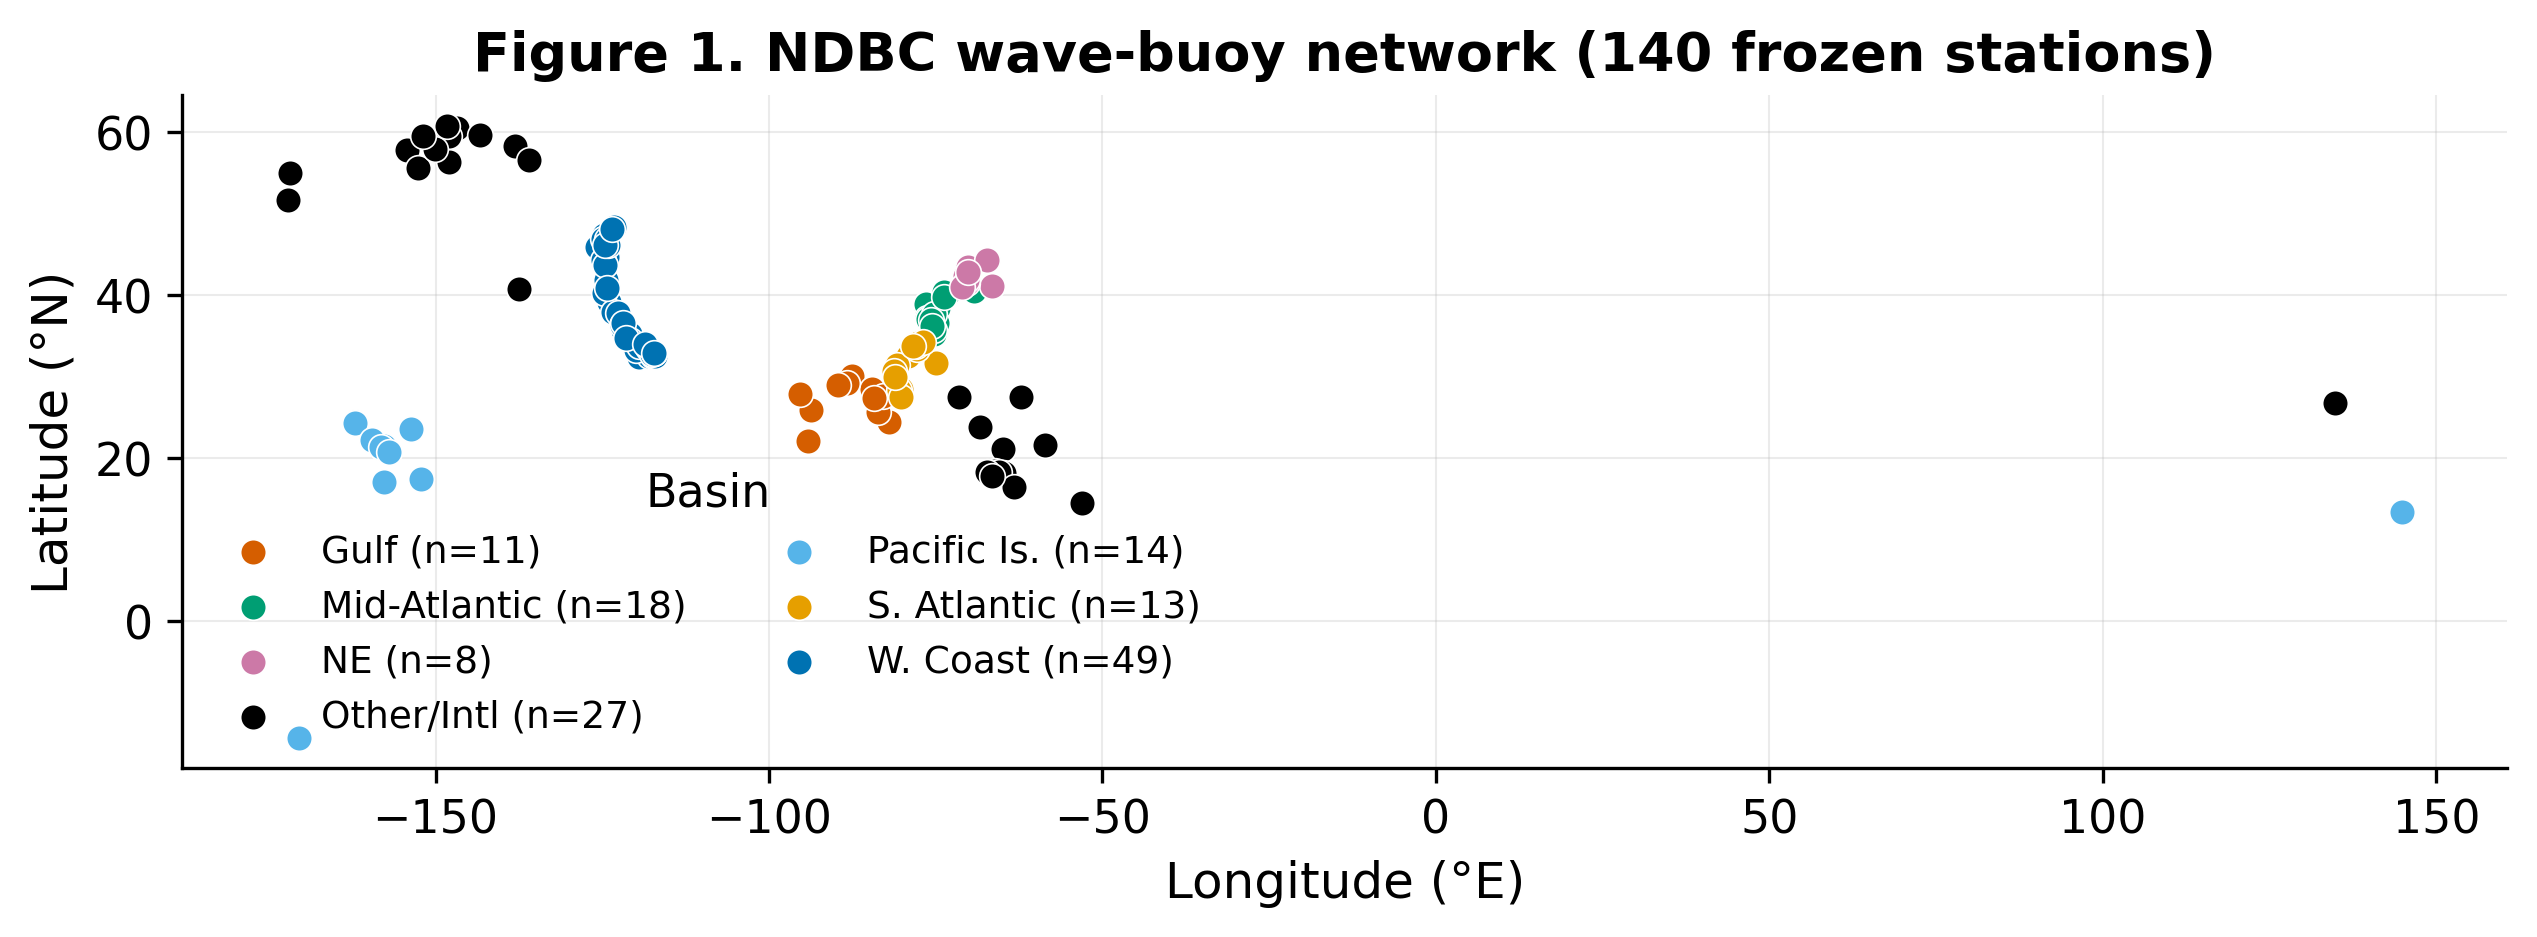
\includegraphics[width=0.86\textwidth]{fig1_station_map.png}
\caption{Selected NDBC stations across U.S. ocean basins after the national
coverage audit and metadata corrections. Nodes are buoys; the panel defines the
spatial domain for the graph.}
\label{fig:map}
\end{figure}

\begin{figure}[t]
\centering
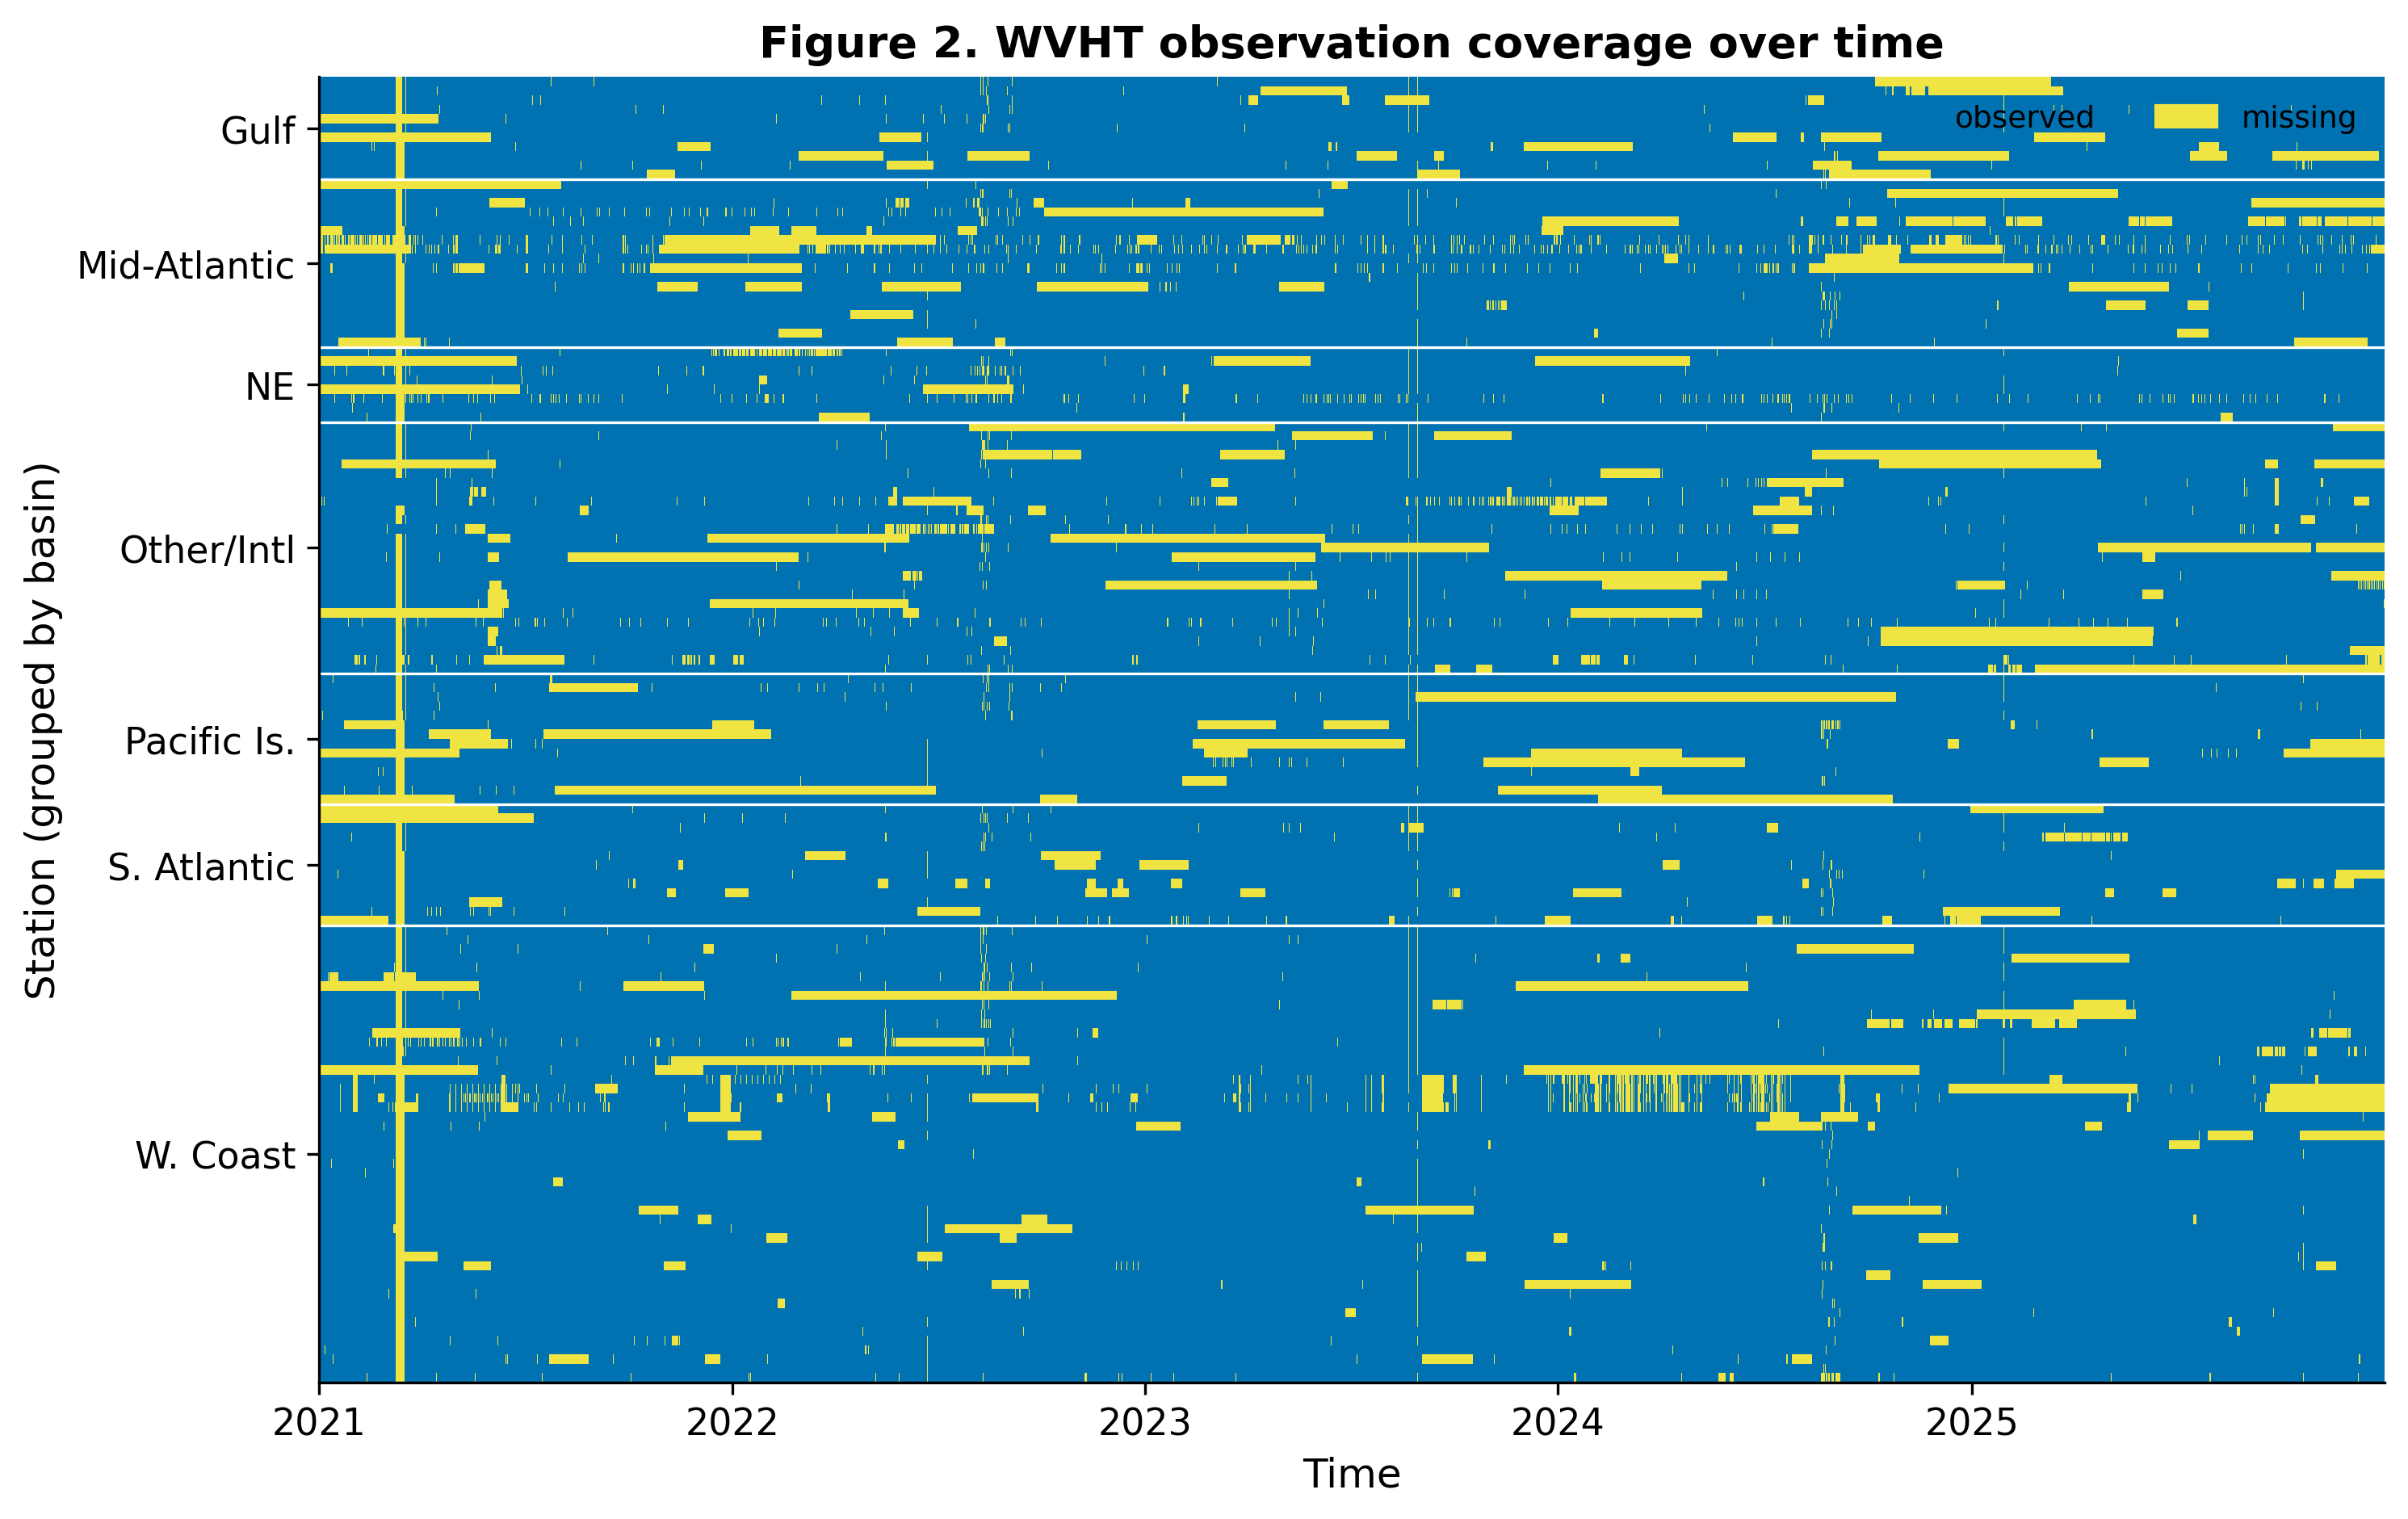
\includegraphics[width=0.86\textwidth]{fig2_missingness.png}
\caption{Missingness structure across stations and time. Gaps are both random
(scattered hourly dropouts) and structured (whole-station outages spanning long
intervals), motivating separate evaluation regimes.}
\label{fig:missing}
\end{figure}

\begin{figure}[t]
\centering
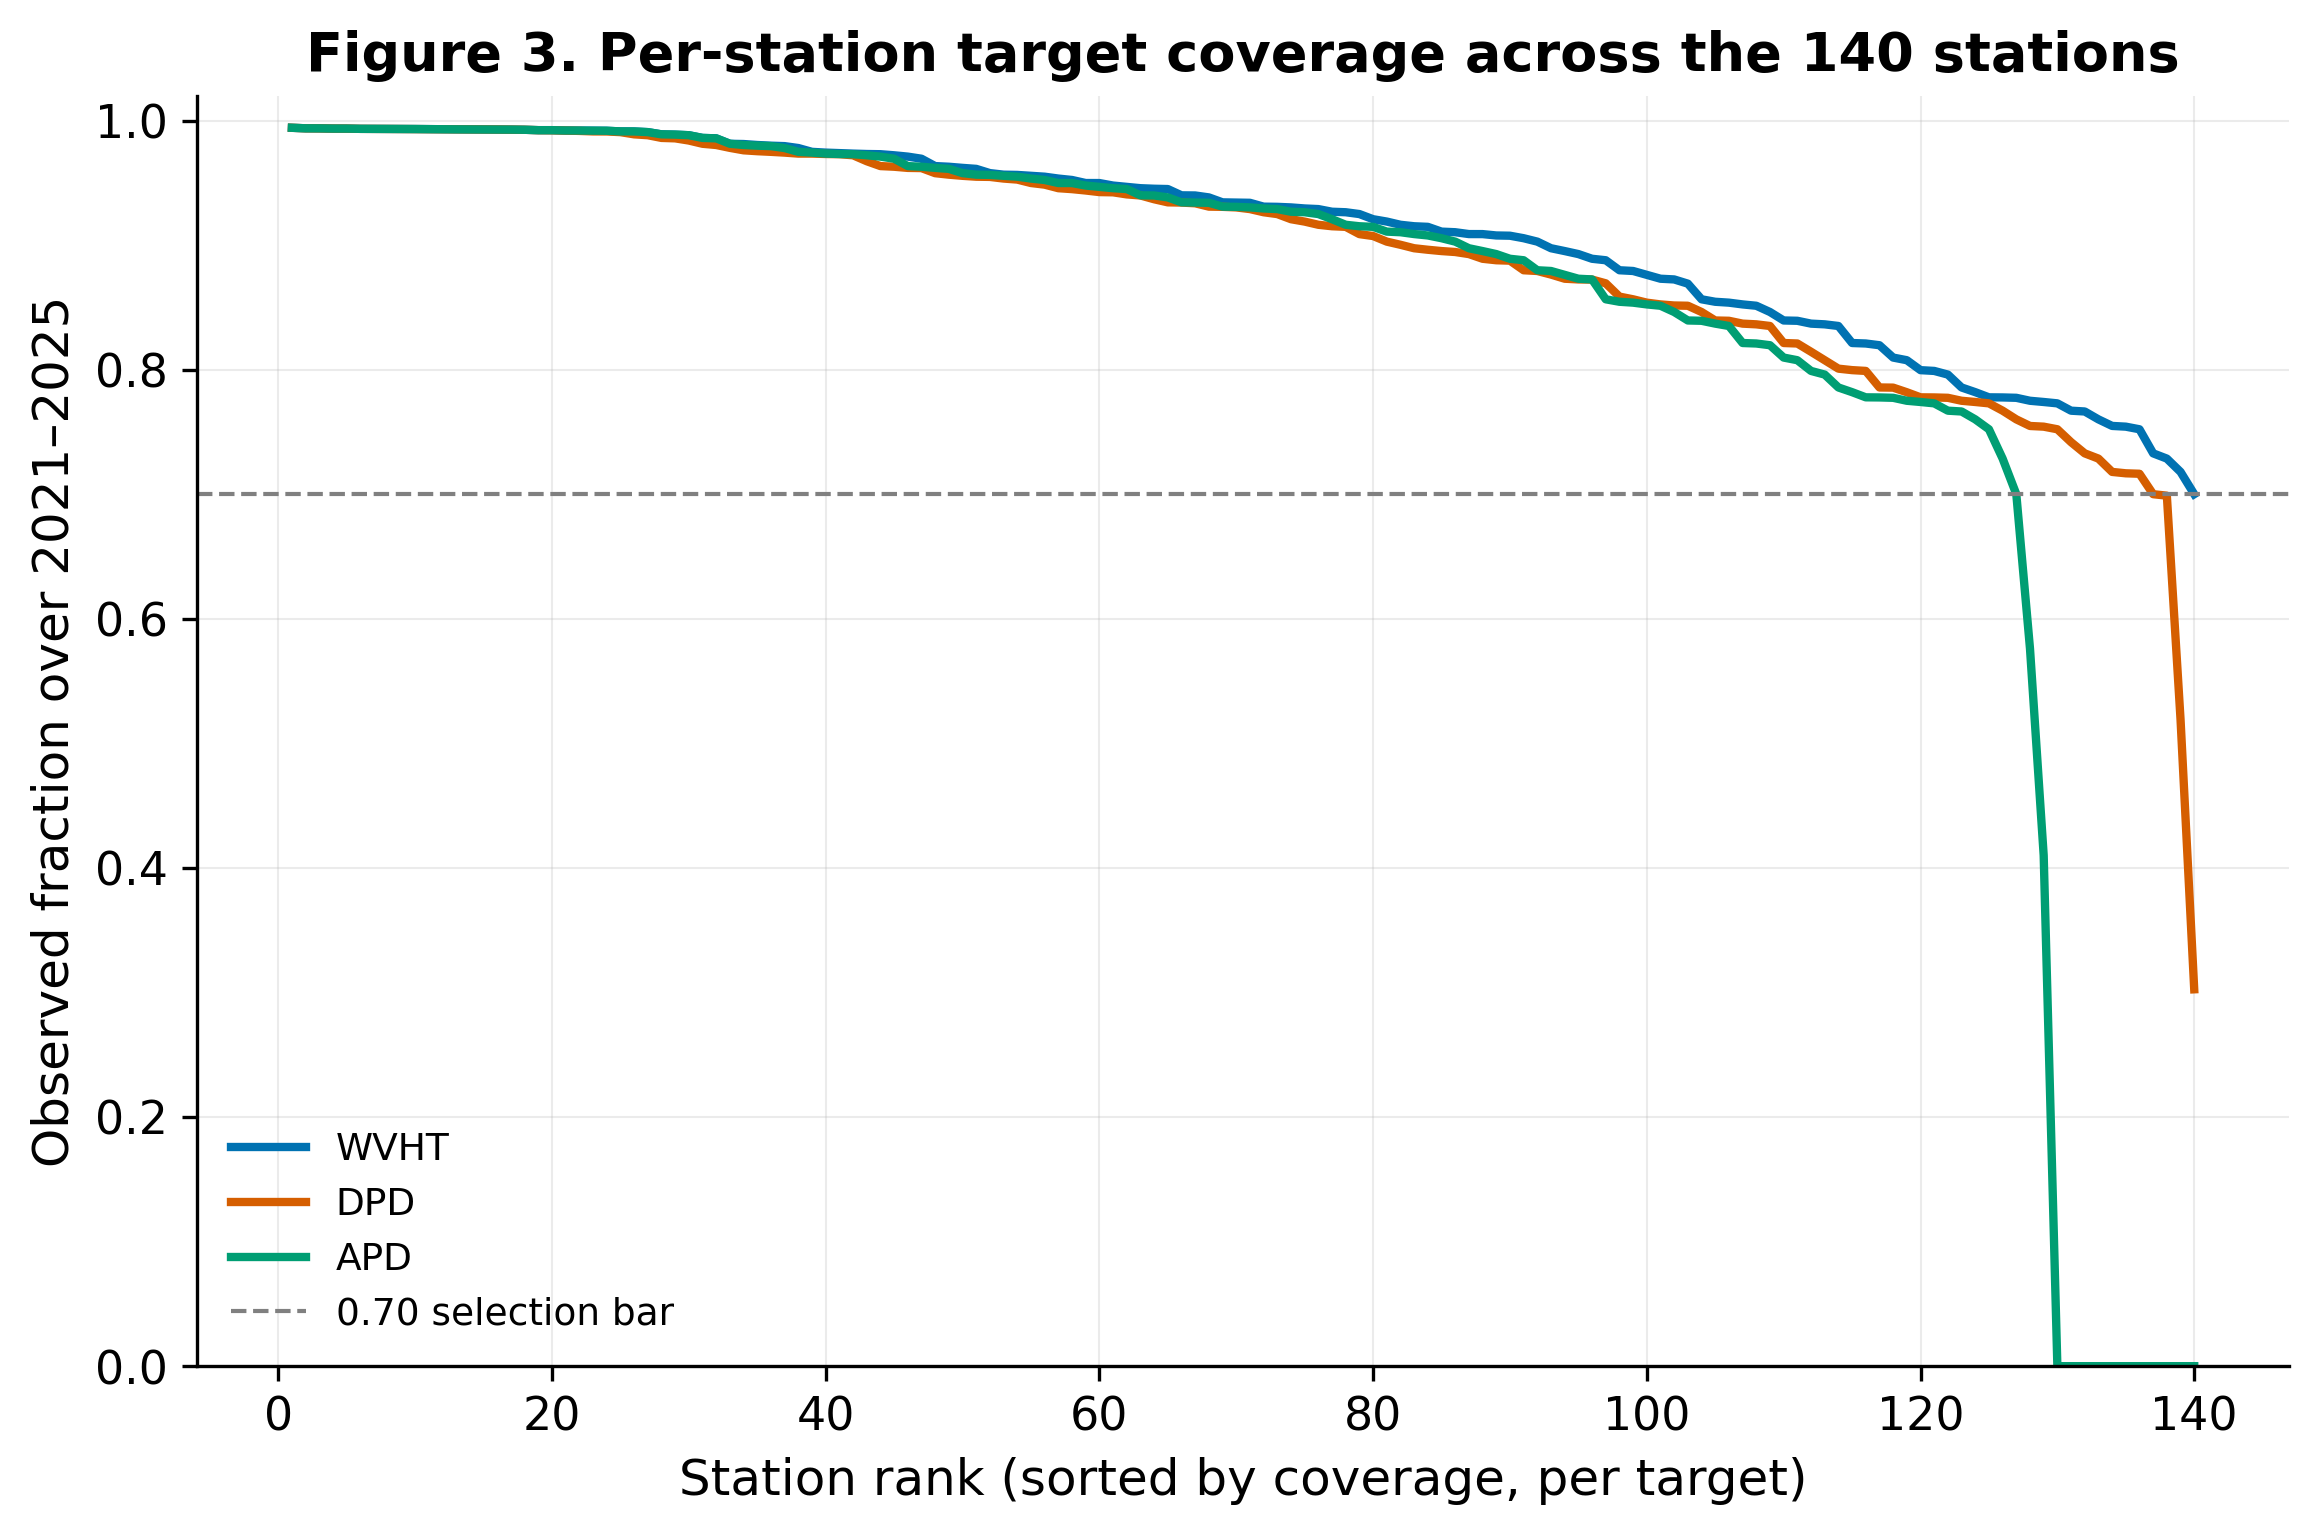
\includegraphics[width=0.72\textwidth]{fig3_coverage_dist.png}
\caption{Distribution of per-station temporal coverage over the study window,
used to set the selection threshold.}
\label{fig:cov}
\end{figure}

\begin{figure}[t]
\centering
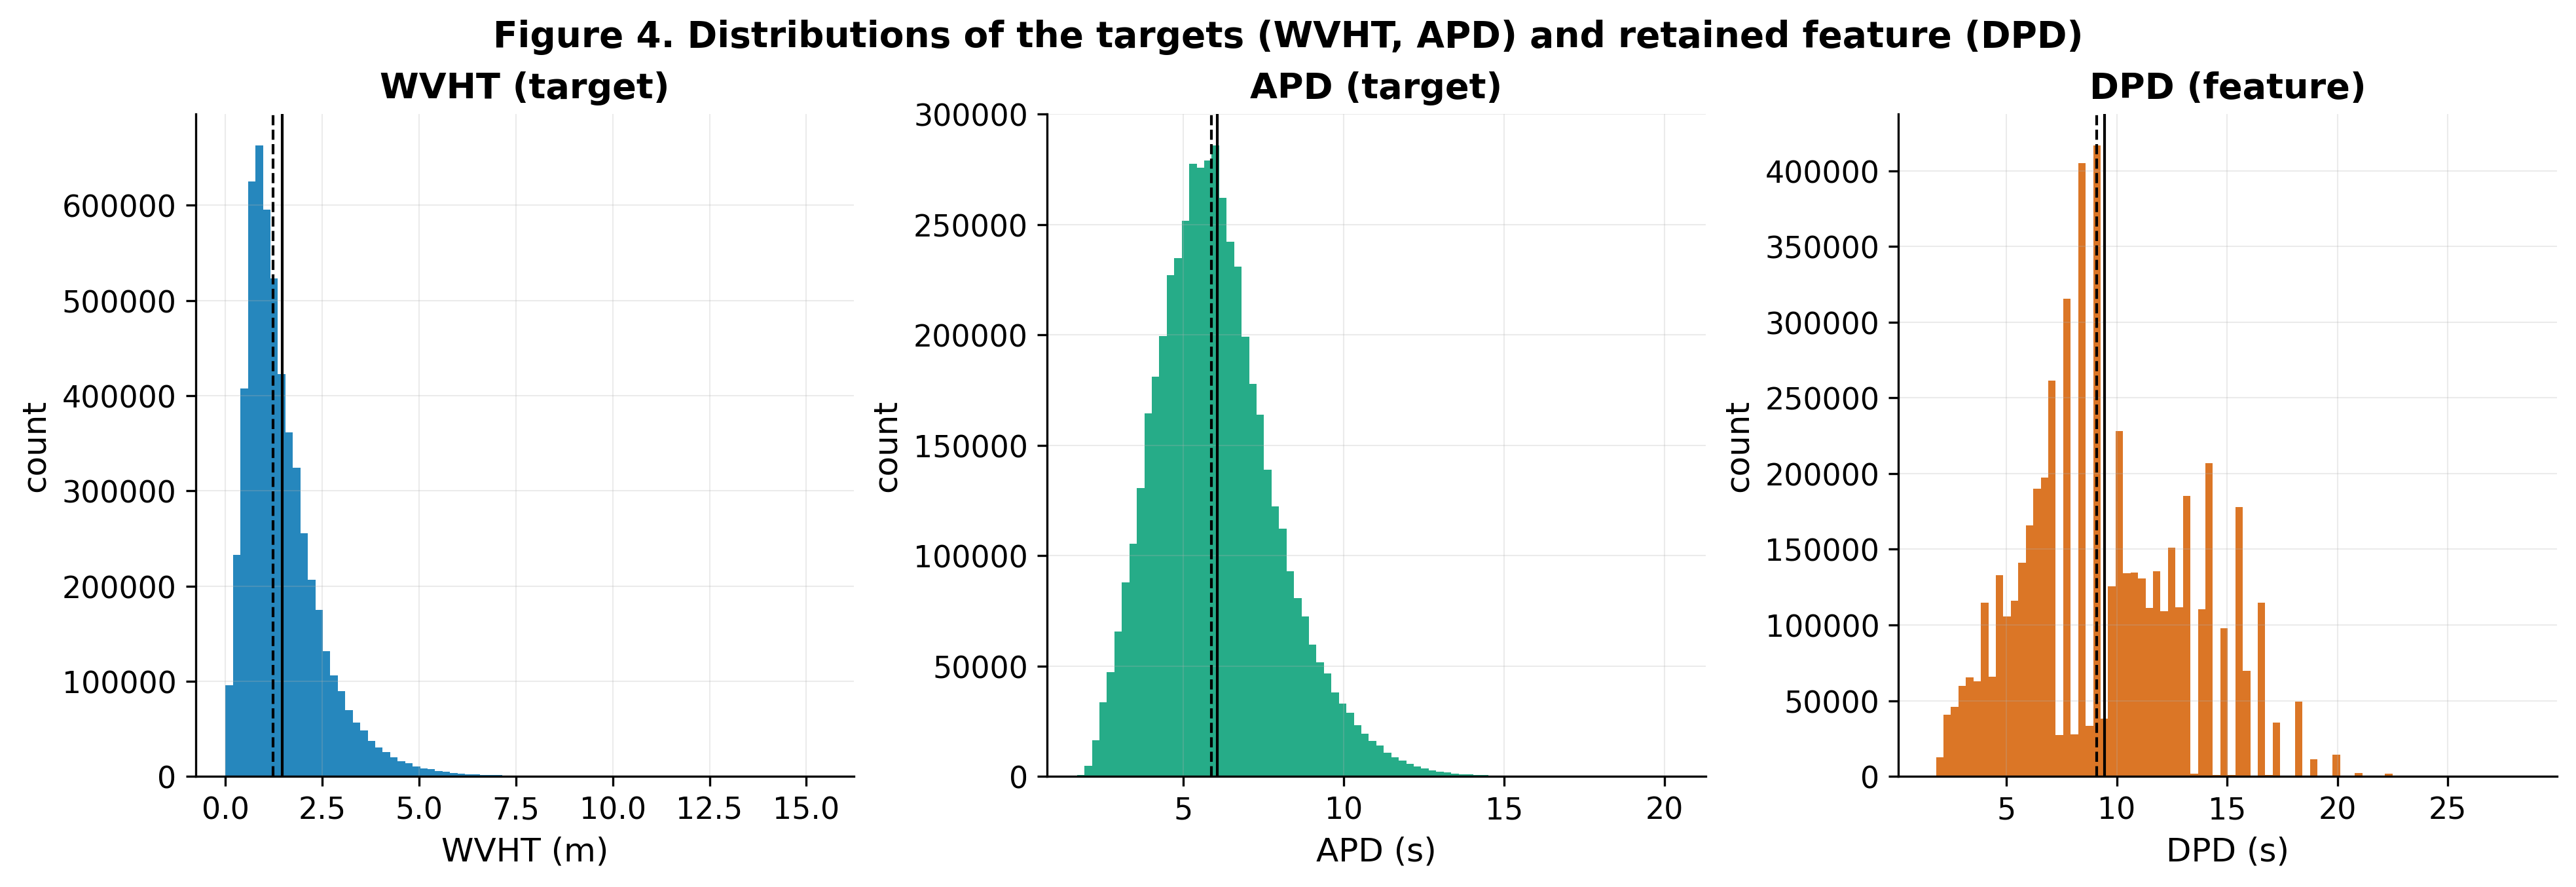
\includegraphics[width=0.86\textwidth]{fig4_target_dists.png}
\caption{Pooled distributions (all stations $\times$ hours) of the two modelled
targets---significant wave height (WVHT) and average wave period (APD)---and the
retained predictor feature, dominant wave period (DPD). DPD is a model input, not
a target. Solid and dashed lines mark the mean and median.}
\label{fig:tdist}
\end{figure}

\begin{figure}[t]
\centering
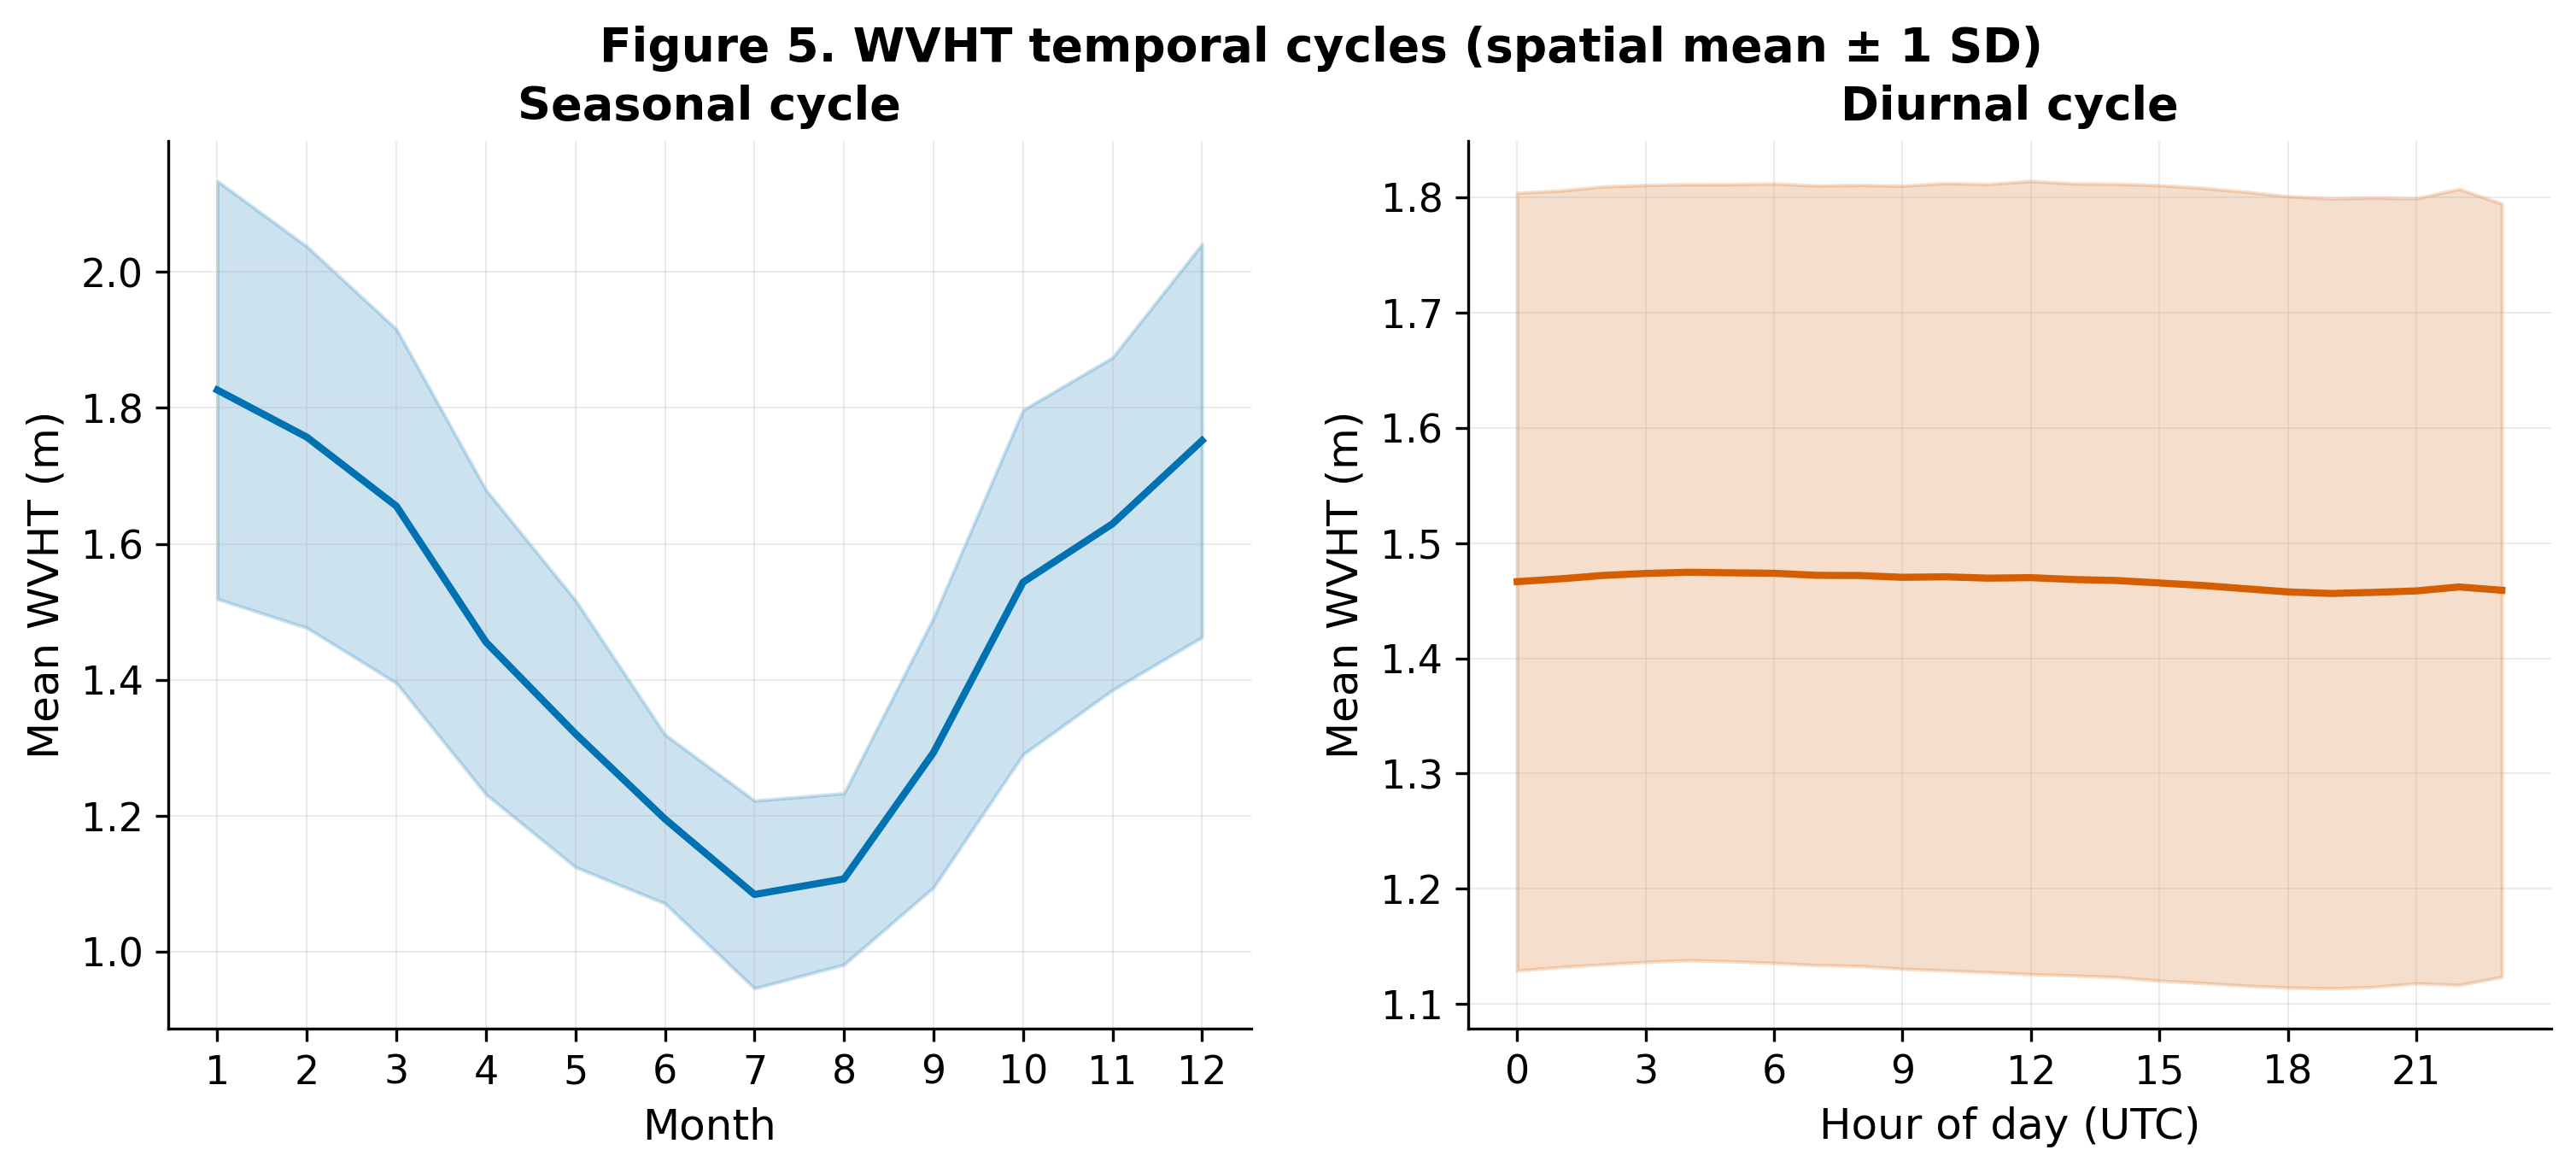
\includegraphics[width=0.86\textwidth]{fig5_temporal_cycles.png}
\caption{Diurnal and seasonal cycles in the targets, showing the temporal
structure available to single-station baselines.}
\label{fig:cycles}
\end{figure}

\begin{figure}[t]
\centering
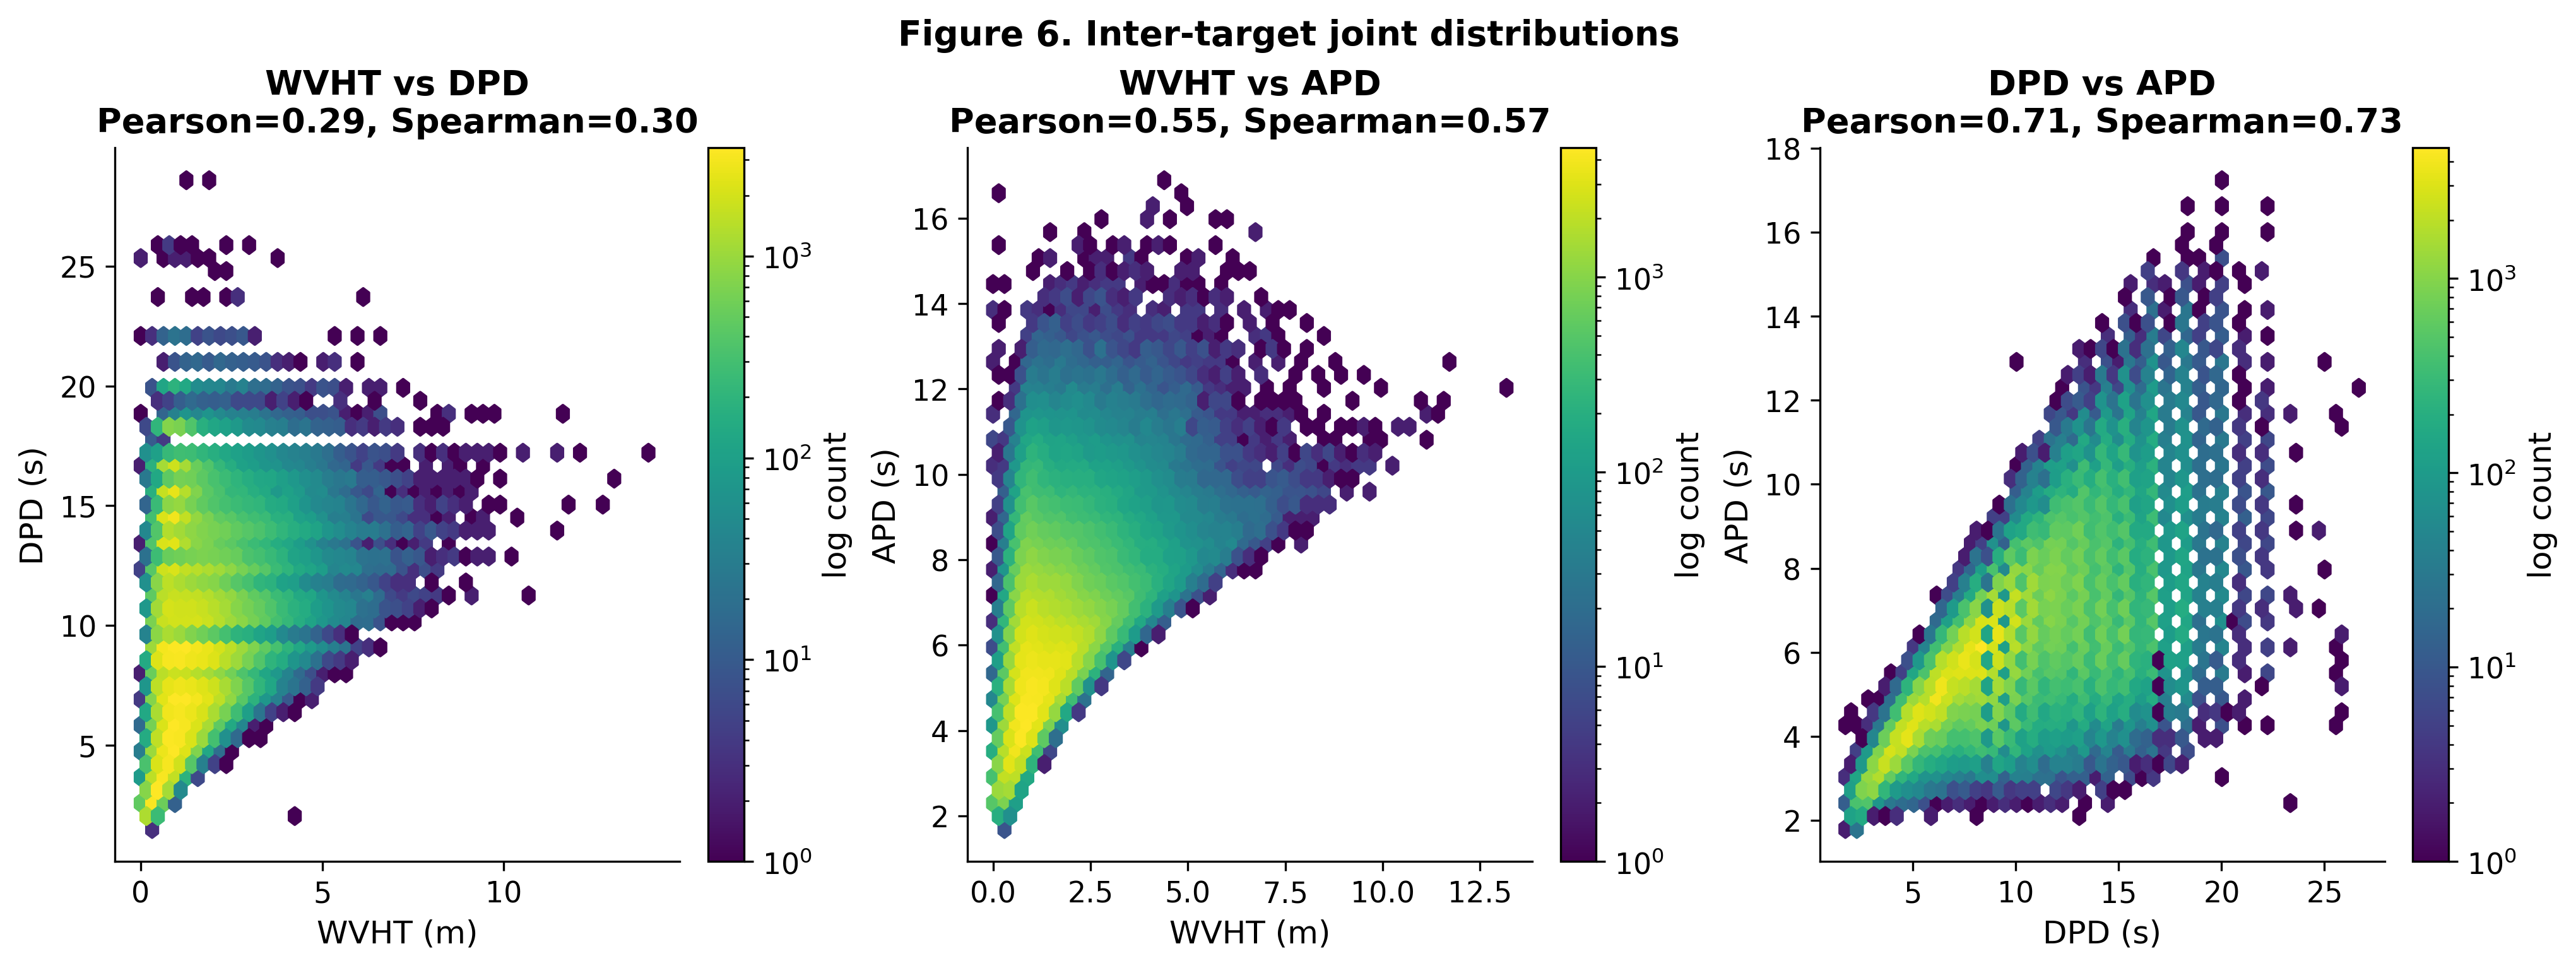
\includegraphics[width=0.72\textwidth]{fig6_target_relationships.png}
\caption{Joint structure of height and period, the relationship the wave-power
computation depends on.}
\label{fig:rel}
\end{figure}

\section{Methodology}
\label{sec:method}

\subsection{Spatiotemporal tensor}
We arrange the data as a tensor $X \in \mathbb{R}^{T \times N \times F}$ of $T$
hourly steps, $N$ stations, and $F$ features (the targets plus retained
covariates). A binary mask $M$ of the same shape marks genuinely observed
entries. All models see $X$ and $M$; no model is allowed to treat an imputed or
padded value as if it were observed.

\subsection{Graph construction}
We connect stations with a $k$-nearest-neighbour graph in geographic distance
($k=8$). Edge weights follow a self-tuning Gaussian kernel,
$w_{ij} = \exp\!\big(-d_{ij}^{2}/(\sigma_i \sigma_j)\big)$, where $\sigma_i$ is
the distance from station $i$ to its $k$-th neighbour. This local scaling avoids
the numerical underflow that a single global bandwidth produces when station
spacing varies by orders of magnitude across basins. We also build a
\emph{basin-aware} variant that zeros edges crossing basin boundaries, to test
whether forbidding cross-basin message passing helps. Figures~\ref{fig:corrdist}
and~\ref{fig:graph} show the empirical correlation--distance decay and the
resulting graph.

\begin{figure}[t]
\centering
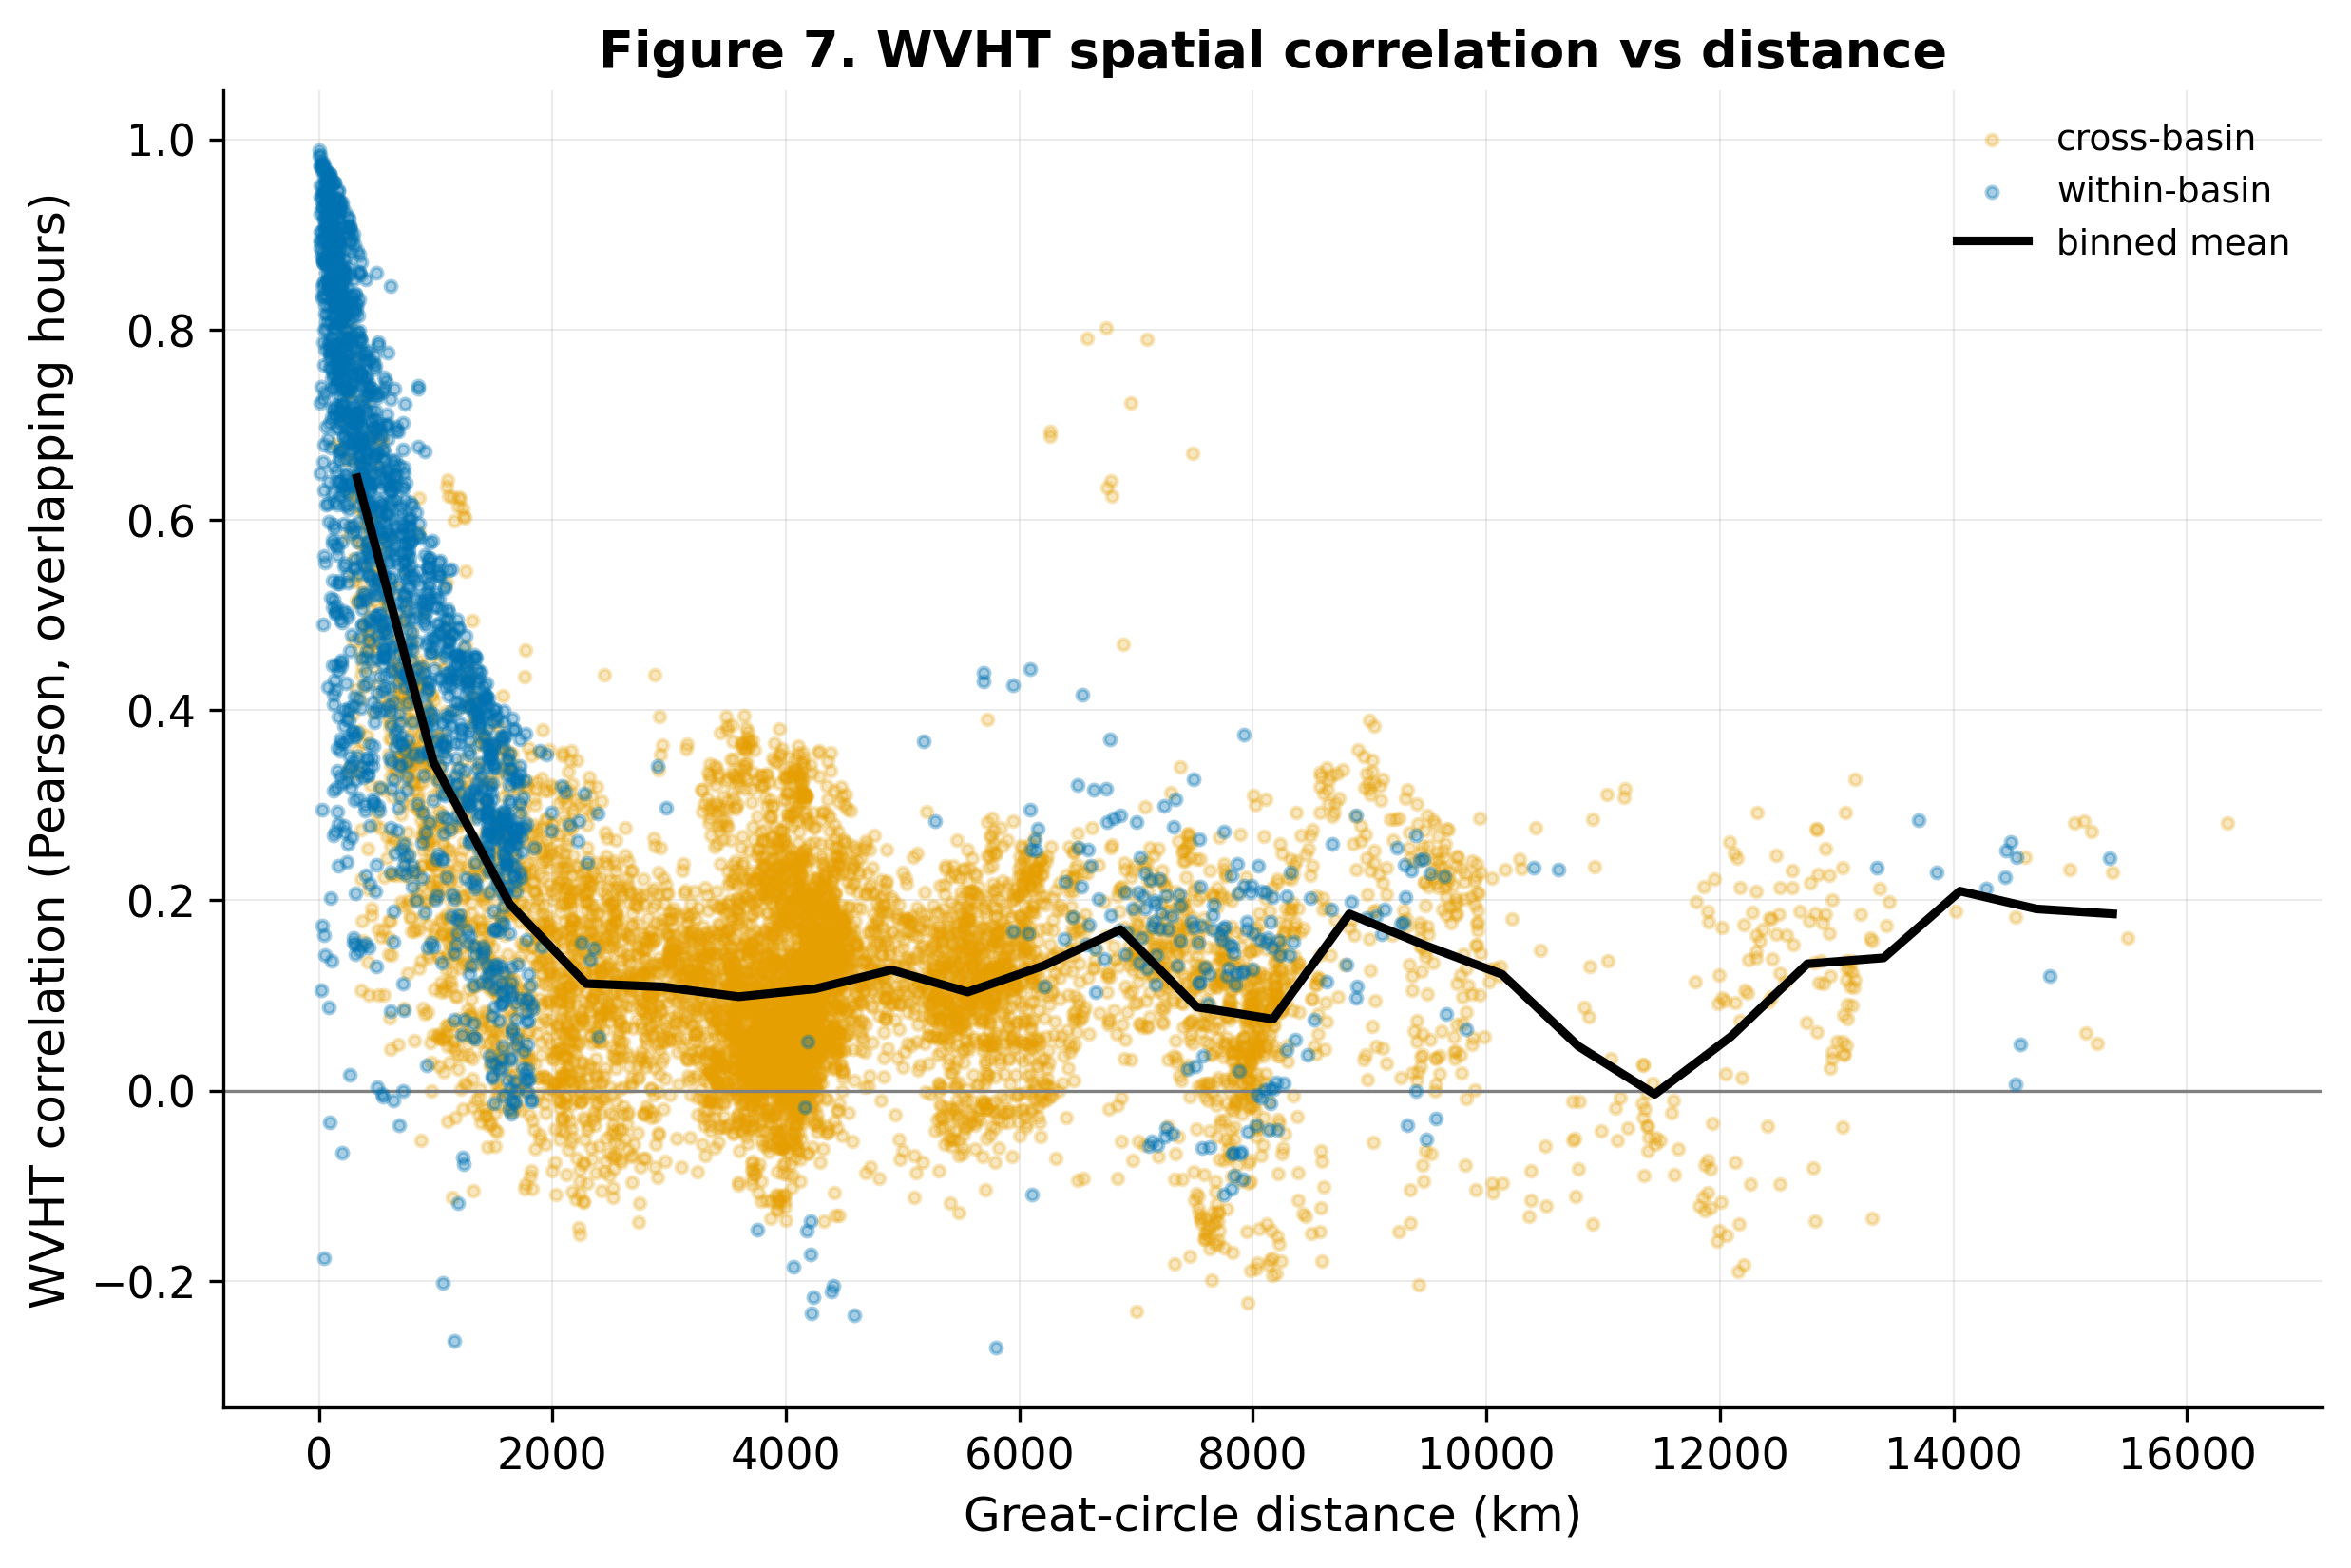
\includegraphics[width=0.72\textwidth]{fig7_corr_distance.png}
\caption{Inter-station target correlation as a function of separation distance.
Correlation decays with distance, justifying a distance-weighted neighbourhood.}
\label{fig:corrdist}
\end{figure}

\begin{figure}[t]
\centering
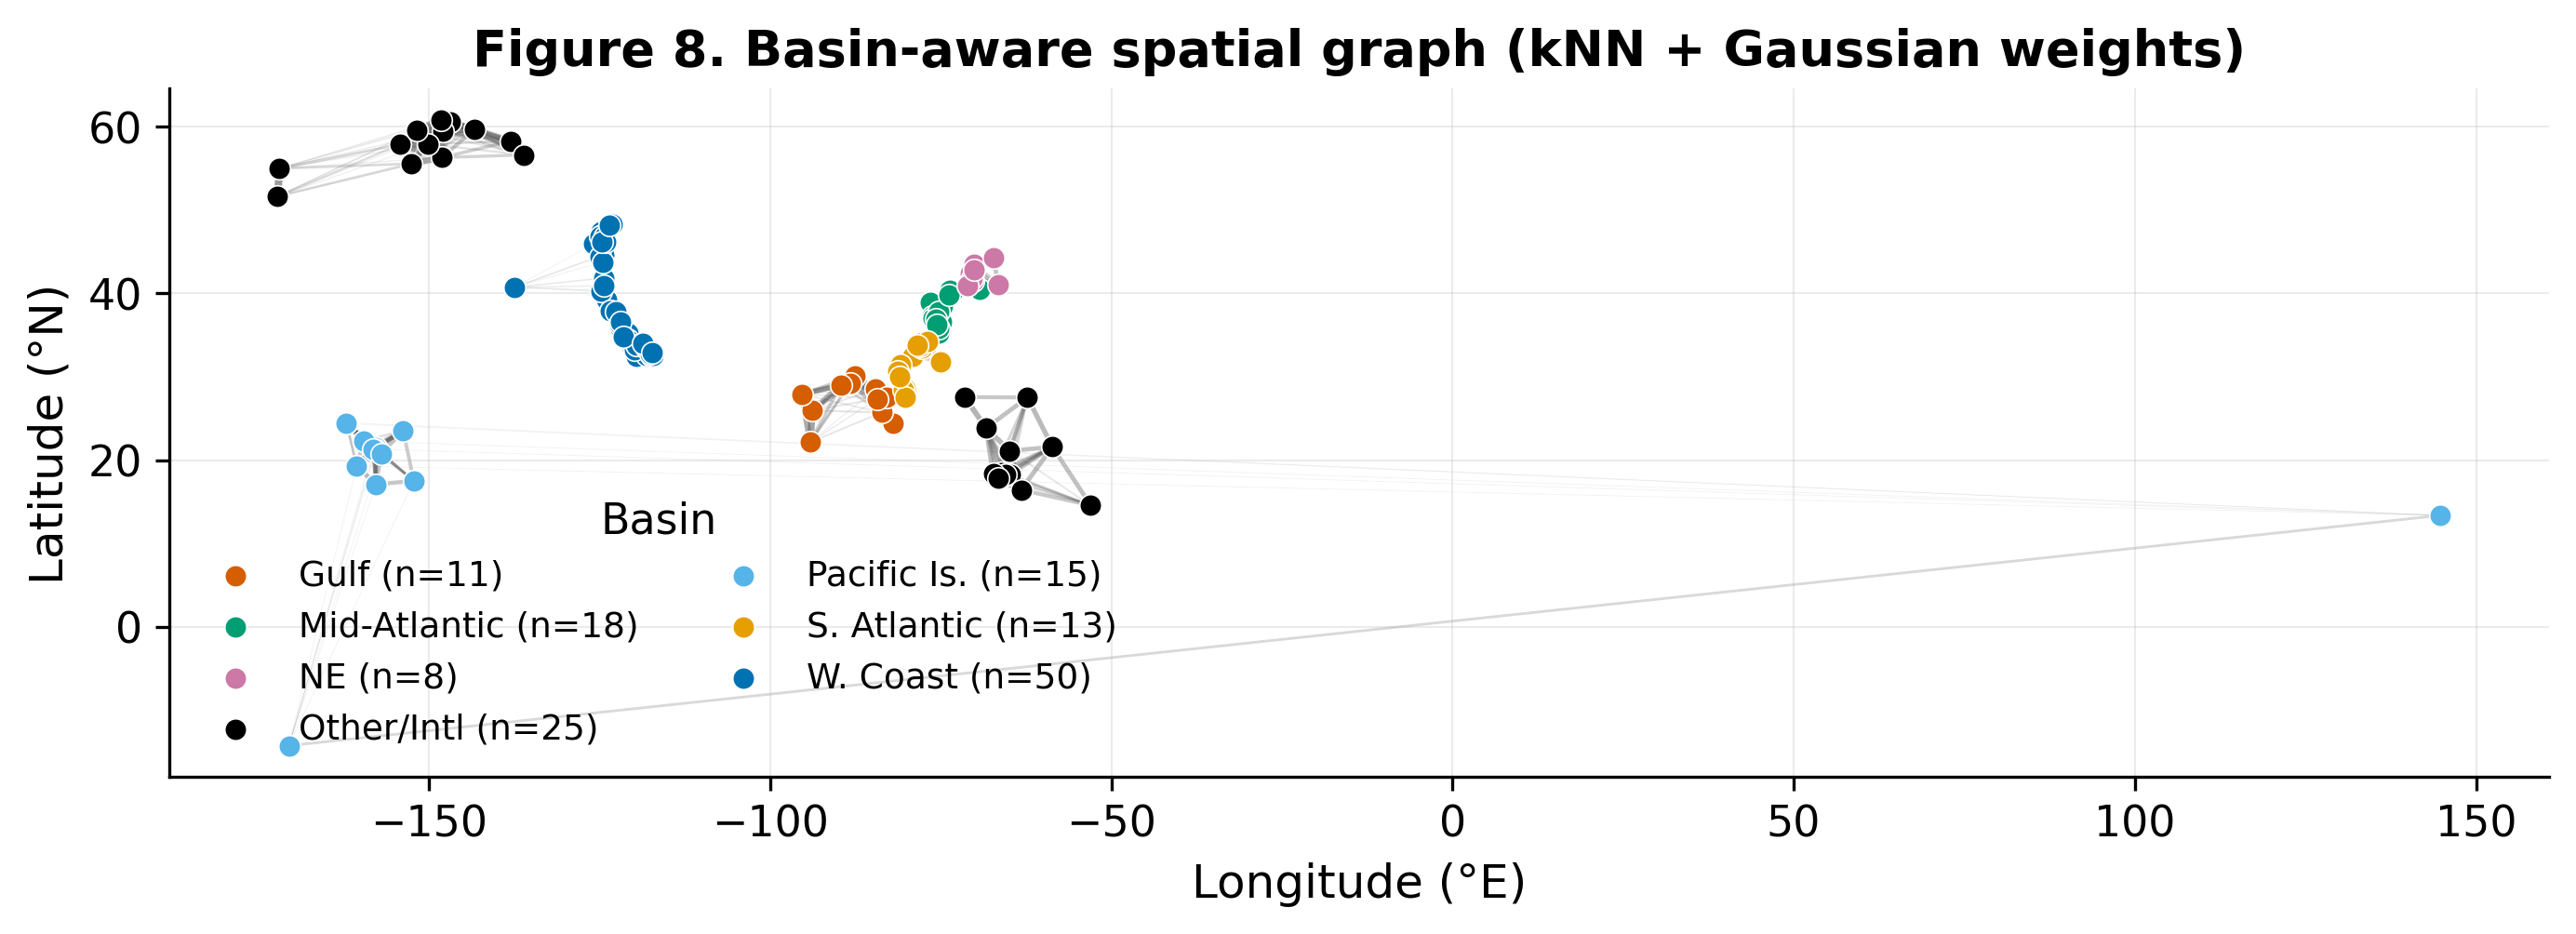
\includegraphics[width=0.86\textwidth]{fig8_spatial_graph.png}
\caption{The $k$-nearest-neighbour Gaussian station graph. Edge shading encodes
the self-tuning kernel weight; the basin-aware variant removes cross-basin
edges.}
\label{fig:graph}
\end{figure}

\subsection{Leakage-safe hide-and-recover protocol}
For imputation we hide observed entries, ask each model to recover them, and
score only on the hidden-but-known cells. We define two regimes. The
\emph{spatial} regime removes whole stations for extended intervals
(station-outage), so a model can only recover a victim from its neighbours and
its own surrounding history. The \emph{temporal} regime removes values within
otherwise-present stations, either completely at random (MCAR) or in contiguous
blocks, at 10\%, 30\%, and 50\% rates. Scoring is confined to truly held-out
cells, and no target leaks through the covariates.

\subsection{Imputation models}
We compare (i) simple baselines---mean fill, forward fill, and linear
interpolation; (ii) spatial baselines---inverse-distance weighting (IDW) and a
combined spatial-plus-temporal interpolator; (iii) SAITS, a self-attention
imputer \citep{saits}; (iv) BRITS, a bidirectional recurrent imputer
\citep{brits}; and (v) GRIN, a graph recurrent imputer \citep{grin}. GRIN is
bidirectional, which is legitimate for imputation because the task is
reconstruction of an interior gap from both sides.

\subsection{Forecasting models and the causal-input design}
Forecasting must respect the arrow of time. We use an input window of
$L=24$~hours and predict targets $h$ steps ahead. Baselines are persistence
(repeat the last value), seasonal-naive (repeat the value one day earlier), and a
per-station autoregressive model, AR(24), fit by least squares as a direct
$h$-step predictor. Our graph model is Graph WaveNet \citep{gwn}.

To avoid leakage we separate training and test information sources. The model is
\emph{trained} on a graph-completed tensor---missing training entries filled by
GRIN, where bidirectional filling is acceptable because it is confined to the
training period. At \emph{test} time the model reads only causal,
forward-filled inputs that use past information alone, and we evaluate only at
origins where the entire input window and the target at $t+h$ are genuinely
observed (a valid-origin mask). This keeps future information out of every test
forecast.

\subsection{Wave-energy computation}
We convert forecasts to deep-water wave power \citep{guillou2020},
\begin{equation}
P \;=\; \frac{\rho g^{2}}{64\pi}\, H_{m0}^{2}\, T_e \;\approx\; 0.49\, H^{2}\, T_e
\quad \text{(kW/m)},
\label{eq:power}
\end{equation}
with $H$ in metres and $T_e$ in seconds. Because NDBC reports APD rather than the
energy period $T_e$, we set $T_e = \alpha \cdot \text{APD}$ with $\alpha = 1.12$,
the JONSWAP-spectrum ratio analysed by \citet{cahill2014}; $\alpha$ is an
explicit configuration parameter. True energy uses observed WVHT and APD at
$t+h$, and a station-hour is scored only where \emph{both} targets are genuinely
observed. Since $\alpha$ multiplies every method's energy identically, method
rankings and persistence-normalized skill are invariant to $\alpha$; only the
absolute kW/m magnitudes depend on it.

\section{Experimental Setup}
\label{sec:setup}
\textbf{Splits.} We train on 2021--2023, validate on 2024, and test on 2025, so
no test period is ever seen during fitting.

\noindent\textbf{Masking.} MCAR and block masks are applied at 10/30/50\% rates;
station-outage masks remove a fixed set of victim stations. To measure
variability we repeat each masked evaluation over three model seeds and, for the
deep models, average within a run before taking the standard deviation across
seeds, so error bars reflect model-training variability rather than mask
resampling.

\noindent\textbf{Metrics.} We report MAE and RMSE in physical units (m for WVHT,
s for APD, kW/m for power) and a persistence-normalized skill,
$\text{skill} = 1 - \text{MAE}_{\text{model}}/\text{MAE}_{\text{persistence}}$,
so that positive values mean ``better than persistence.''

\noindent\textbf{Hyperparameters and compute.} Deep models are seeded
(seed~0) and checkpointed. GRIN is trained with a capped budget (up to 50 epochs,
early stopping with patience 10). Graph WaveNet is trained for 30 epochs on CPU:
its channels-last convolution is unsupported on the Apple MPS backend, and we
observed that sustained multi-day MPS load degrades throughput, so CPU is used
for reproducibility. All runs use a fixed software stack
(\texttt{tsl}~\citep{tsl}, \texttt{PyPOTS}~\citep{pypots},
PyTorch~\citep{pytorch}, PyTorch~Geometric~\citep{pyg}).

\section{Results}
\label{sec:results}

\subsection{Imputation}
Table~\ref{tab:imp} reports imputation MAE for both targets in three
representative regimes. GRIN achieves the lowest error wherever the missing gaps
are \emph{structured}. Under whole-station outages it recovers WVHT at
0.346$\pm$0.007~m, far below the best spatial baseline (IDW, 0.443~m) and
the spatial-plus-temporal interpolator (0.426~m), and well below the
purely temporal deep models (SAITS 0.743~m, BRITS 0.727~m)
whose single-station design cannot see a station that is entirely absent. It is
also best under 50\% contiguous-block missingness for both targets. The picture
changes only under 50\% \emph{completely random} missingness: isolated single-hour
gaps are easy to interpolate, so linear interpolation attains the lowest error
(WVHT 0.074~m) and GRIN (0.082~m) is competitive---matching
or slightly beating the attention model SAITS (0.086~m) on height---
rather than dominant. The message is not that GRIN dominates everywhere, but that
it is best exactly where spatial or temporal structure must be exploited, and
merely competitive where a gap is trivial to fill.

\begin{table}[t]
\centering
\caption{Imputation mean absolute error (lower is better). Station-outage is the
spatial regime; MCAR-50\% and Block-50\% are temporal regimes. GRIN values are
mean $\pm$ standard deviation over three model seeds. Best per column in bold.}
\label{tab:imp}
\small
\begin{tabular}{l cc cc cc}
\toprule
& \multicolumn{2}{c}{Station-outage} & \multicolumn{2}{c}{MCAR-50\%}
& \multicolumn{2}{c}{Block-50\%}\\
\cmidrule(lr){2-3}\cmidrule(lr){4-5}\cmidrule(lr){6-7}
Method & WVHT & APD & WVHT & APD & WVHT & APD\\
\midrule
Mean fill & 0.458 & 0.955 & 0.476 & 0.997 & 0.445 & 0.968 \\
Forward fill & 0.637 & 1.303 & 0.111 & 0.306 & 0.702 & 1.410 \\
Linear interp & 0.637 & 1.303 & \textbf{0.074} & \textbf{0.211} & 0.557 & 1.186 \\
Spatial IDW & 0.443 & 0.765 & 0.430 & 0.844 & 0.437 & 0.889 \\
Spatial+temporal & 0.426 & 0.846 & 0.229 & 0.462 & 0.392 & 0.857 \\
SAITS & 0.743 & 1.694 & 0.086 & 0.214 & 0.598 & 0.809 \\
BRITS & 0.727 & 1.572 & 0.123 & 0.386 & 0.682 & 1.055 \\
GRIN & \textbf{0.346$\pm$0.007} & \textbf{0.726$\pm$0.033} & 0.082$\pm$0.002 & 0.228$\pm$0.002 & \textbf{0.373$\pm$0.021} & \textbf{0.704$\pm$0.039} \\
\bottomrule
\end{tabular}
\end{table}

\paragraph{Isolating the graph's contribution.}
Comparing GRIN against SAITS station by station isolates the effect of adding
spatial message passing to a strong temporal model. Averaged over victim
stations, GRIN reduces station-outage error by about 0.38~m in WVHT and
0.86~s in APD relative to SAITS. This gap is the graph's specific
contribution: the two models share the deep-learning machinery, and only GRIN
uses neighbours.

\paragraph{Does station connectivity predict recovery?}
If the graph is the reason GRIN recovers outages, better-connected stations
should be easier to recover. Table~\ref{tab:conn} tests this with Spearman
correlations between three connectivity measures and recovery error, in raw
form, after normalizing by each station's own variability, and as the GRIN-minus-
SAITS advantage. The signs are consistent with the hypothesis---higher degree
and denser edge weight tend to lower normalized error---and several coefficients
reach significance ($^{*}p<0.05$). We deliberately do not overclaim: the sample
is small ($n=38$ victim stations for WVHT and $n=33$ for APD), so we read this
as \emph{suggestive}, directional evidence rather than a firm law.
Figure~\ref{fig:conn} visualizes the relationship.

\begin{table}[t]
\centering
\caption{Spearman correlation between station connectivity and station-outage
recovery. Negative values mean better-connected stations are recovered more
accurately. ``Normalized'' divides error by the station's own variability;
``advantage'' is GRIN minus SAITS. $^{*}p<0.05$. Samples are small
($n=38$ stations for WVHT, $n=33$ for APD), so these are suggestive.}
\label{tab:conn}
\small
\begin{tabular}{l l ccc}
\toprule
Target & Connectivity measure & Raw & Normalized & Advantage\\
\midrule
WVHT & degree & -0.36* & -0.53* & +0.21 \\
WVHT & neighbour dist. & +0.59* & +0.29 & -0.19 \\
WVHT & edge-weight sum & -0.46* & -0.52* & +0.16 \\
APD & degree & +0.26 & -0.35* & +0.16 \\
APD & neighbour dist. & -0.46* & -0.01 & -0.47* \\
APD & edge-weight sum & +0.40* & -0.20 & +0.38* \\
\bottomrule
\end{tabular}
\end{table}

\begin{figure}[t]
\centering
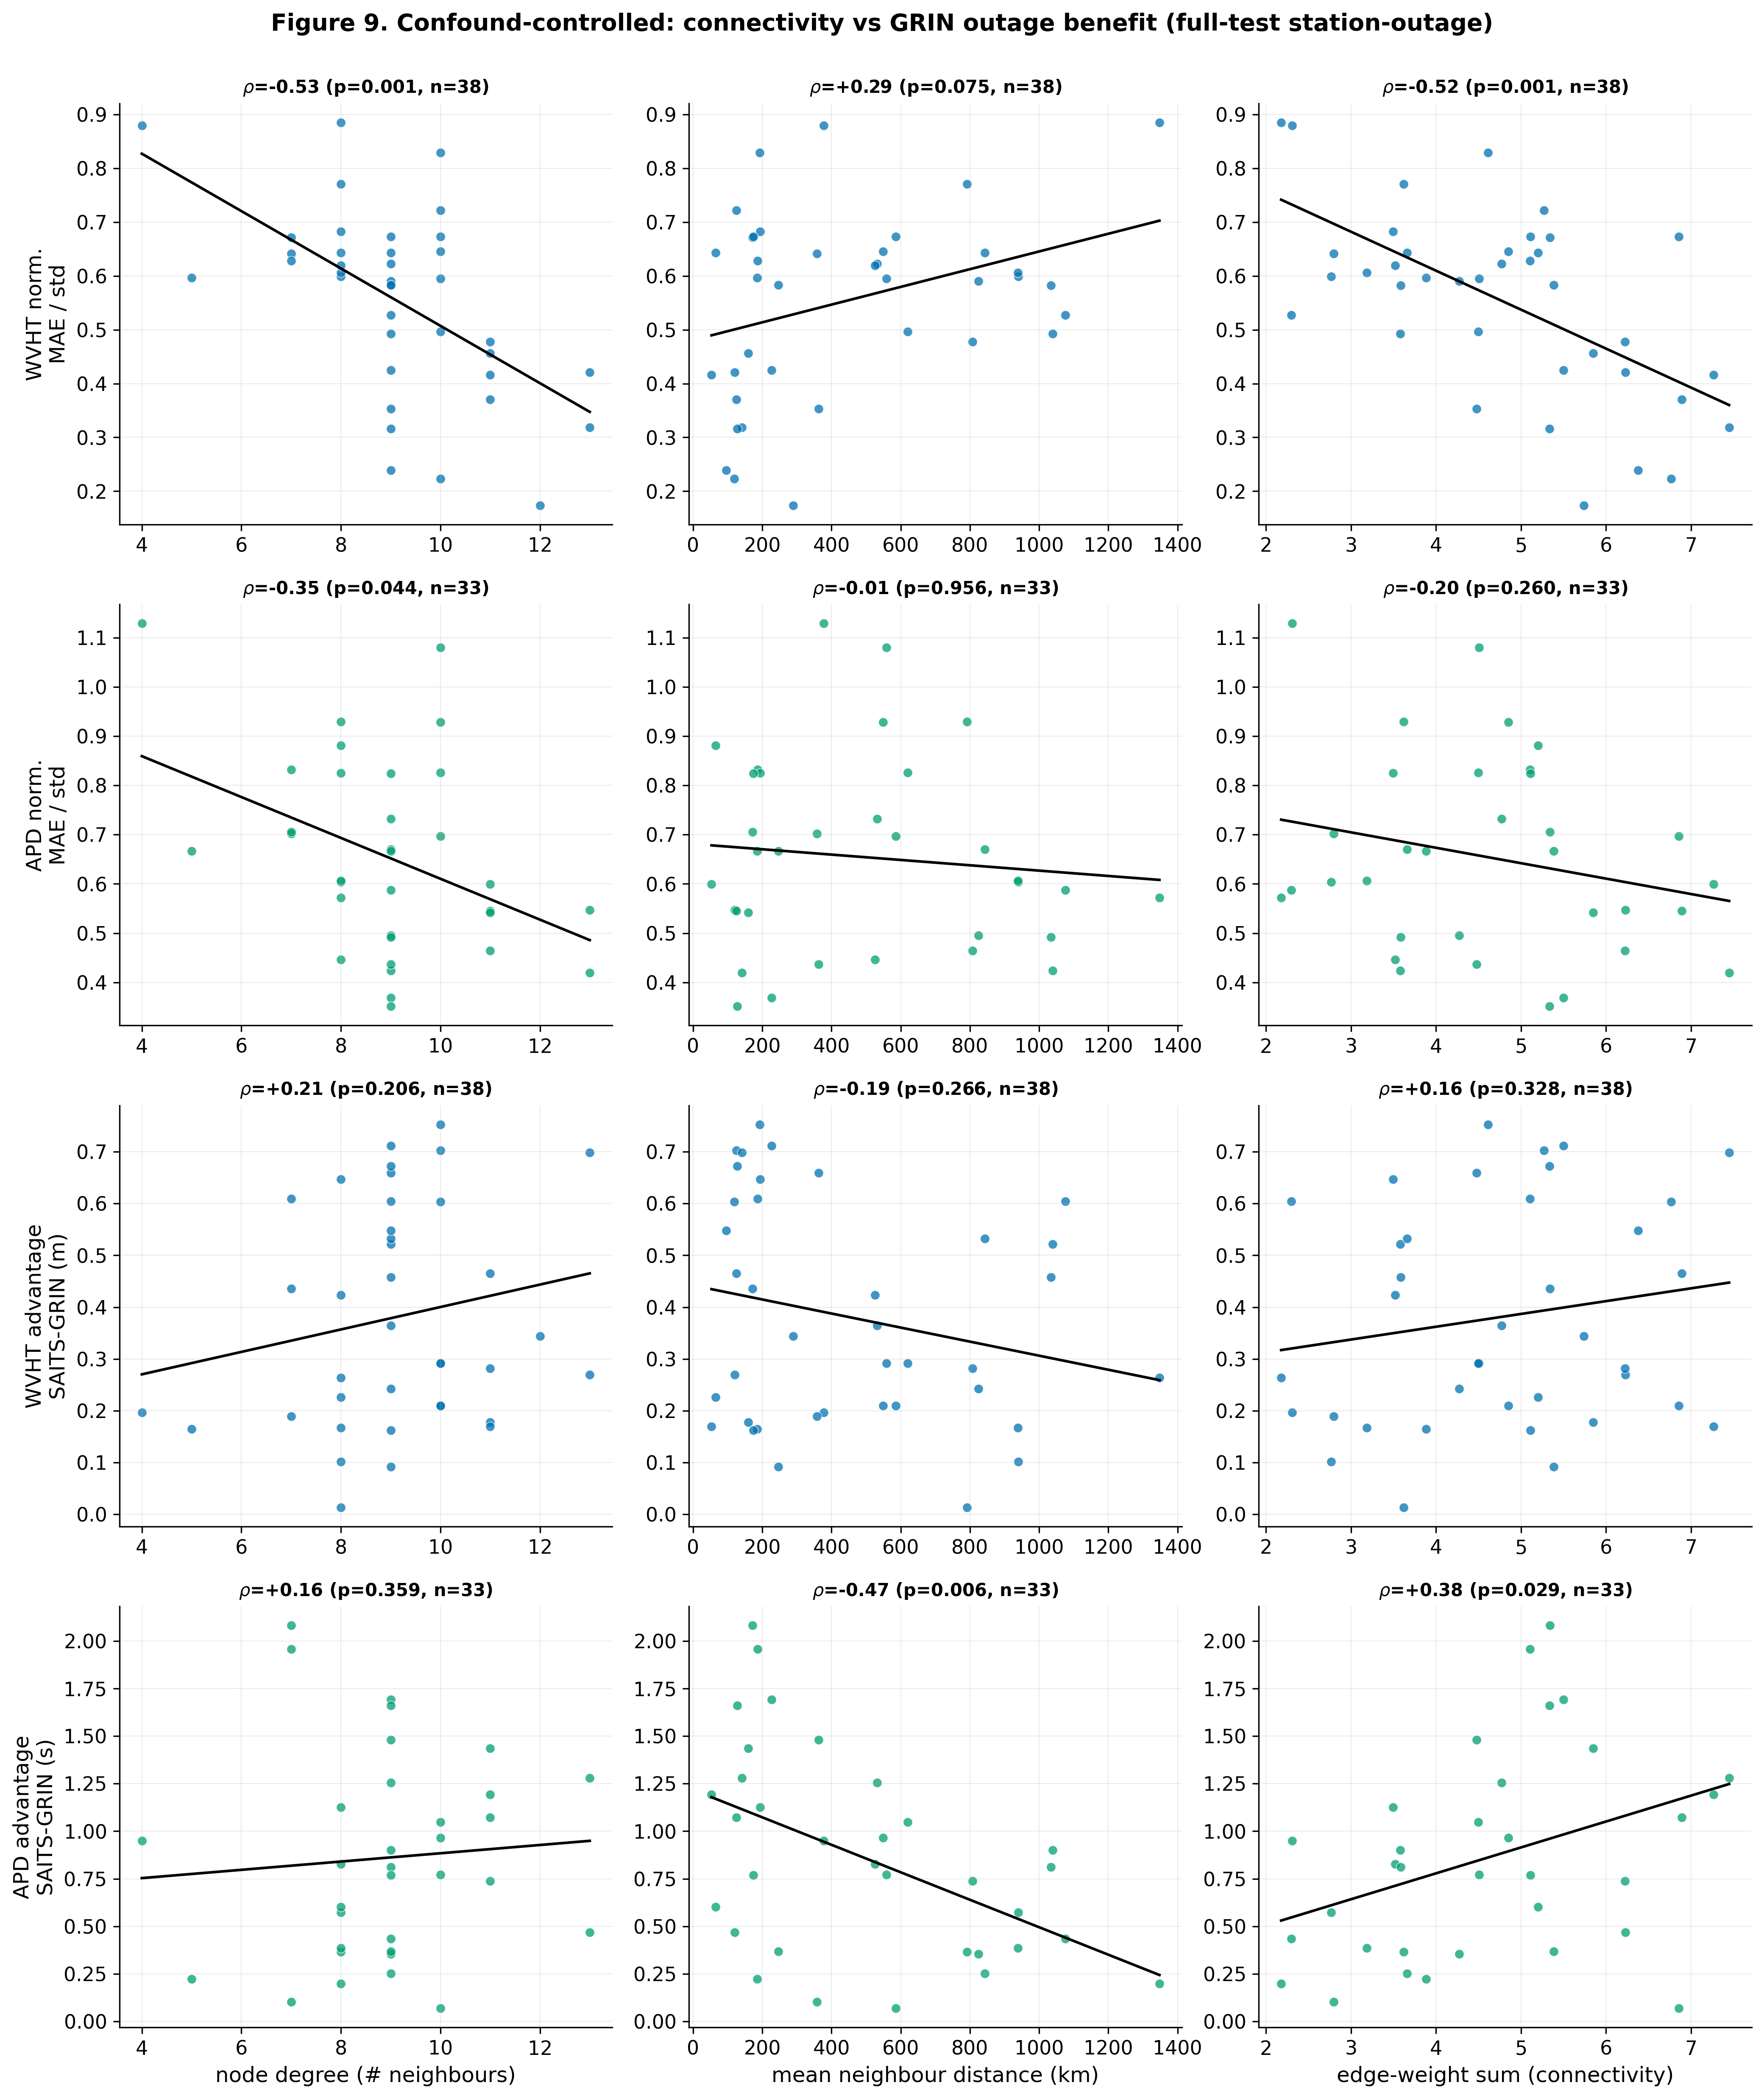
\includegraphics[width=0.86\textwidth]{fig9_connectivity_recovery.png}
\caption{Station-outage recovery error against graph connectivity. Better-
connected stations tend to be recovered more accurately, but the trend is based
on a small sample and is reported as suggestive.}
\label{fig:conn}
\end{figure}

\paragraph{A within-noise negative result: basin-aware edges.}
We expected that forbidding cross-basin message passing would help, since distant
basins share little wave physics. It does not. Table~\ref{tab:abl} compares the
basin-aware graph against the plain $k$-nearest-neighbour graph; in 16
of 16 target-regime cells the difference is smaller than the combined
model-seed noise. We report this as a useful simplification: the plain graph is
adequate, and the extra basin bookkeeping is unnecessary.

\begin{table}[t]
\centering
\caption{Basin-aware versus plain $k$-NN graph (imputation MAE, mean $\pm$
standard deviation over three model seeds). ``Exceeds noise'' is yes only when
the advantage is larger than the combined seed standard deviation.}
\label{tab:abl}
\small
\begin{tabular}{l l cc c c c}
\toprule
Regime & Target & Basin-aware & Plain $k$-NN & Advantage & Seed SD & Exceeds noise\\
\midrule
Station-outage & WVHT & 0.346$\pm$0.007 & 0.340$\pm$0.013 & -0.006 & 0.015 & no \\
Station-outage & APD & 0.726$\pm$0.033 & 0.745$\pm$0.052 & +0.018 & 0.062 & no \\
MCAR-50\% & WVHT & 0.082$\pm$0.002 & 0.083$\pm$0.002 & +0.001 & 0.003 & no \\
MCAR-50\% & APD & 0.228$\pm$0.002 & 0.228$\pm$0.002 & +0.000 & 0.003 & no \\
Block-50\% & WVHT & 0.373$\pm$0.021 & 0.363$\pm$0.015 & -0.010 & 0.026 & no \\
Block-50\% & APD & 0.704$\pm$0.039 & 0.716$\pm$0.032 & +0.012 & 0.050 & no \\
\bottomrule
\end{tabular}
\end{table}

\subsection{Forecasting}
Table~\ref{tab:fc} reports forecast MAE and persistence-normalized skill at
12 and 24~hours. Two findings stand out. First, persistence is extremely strong
at very short range---at 1~hour its WVHT error is only 0.086~m and it is
essentially unbeatable---so we report honestly that the value of a learned model
appears only as the horizon lengthens. Second, at 12--24~hours Graph WaveNet
adds real skill: about +0.158 (WVHT, $h{=}12$) rising to +0.166 at
$h{=}24$, and comparable skill on APD (+0.161 to +0.157). This is roughly
double the autoregressive model, whose WVHT skill is +0.054 at $h{=}12$ and
+0.090 at $h{=}24$. Figure~\ref{fig:horizon} shows how persistence degrades and
how the learned models open a gap as the horizon grows.

\begin{table}[t]
\centering
\caption{Forecast MAE and persistence-normalized skill (in parentheses) at 12
and 24 hours. Persistence is the reference, so its skill is zero by definition.
Higher skill is better.}
\label{tab:fc}
\small
\begin{tabular}{l cc cc}
\toprule
& \multicolumn{2}{c}{WVHT (m)} & \multicolumn{2}{c}{APD (s)}\\
\cmidrule(lr){2-3}\cmidrule(lr){4-5}
Method & $h{=}12$ & $h{=}24$ & $h{=}12$ & $h{=}24$\\
\midrule
Persistence & 0.296 & 0.416 & 0.724 & 0.884 \\
AR(24) & 0.280 (+0.054) & 0.378 (+0.090) & 0.654 (+0.096) & 0.789 (+0.107) \\
GraphWaveNet & 0.249 (+0.158) & 0.347 (+0.166) & 0.607 (+0.161) & 0.745 (+0.157) \\
\bottomrule
\end{tabular}
\end{table}

\begin{figure}[t]
\centering
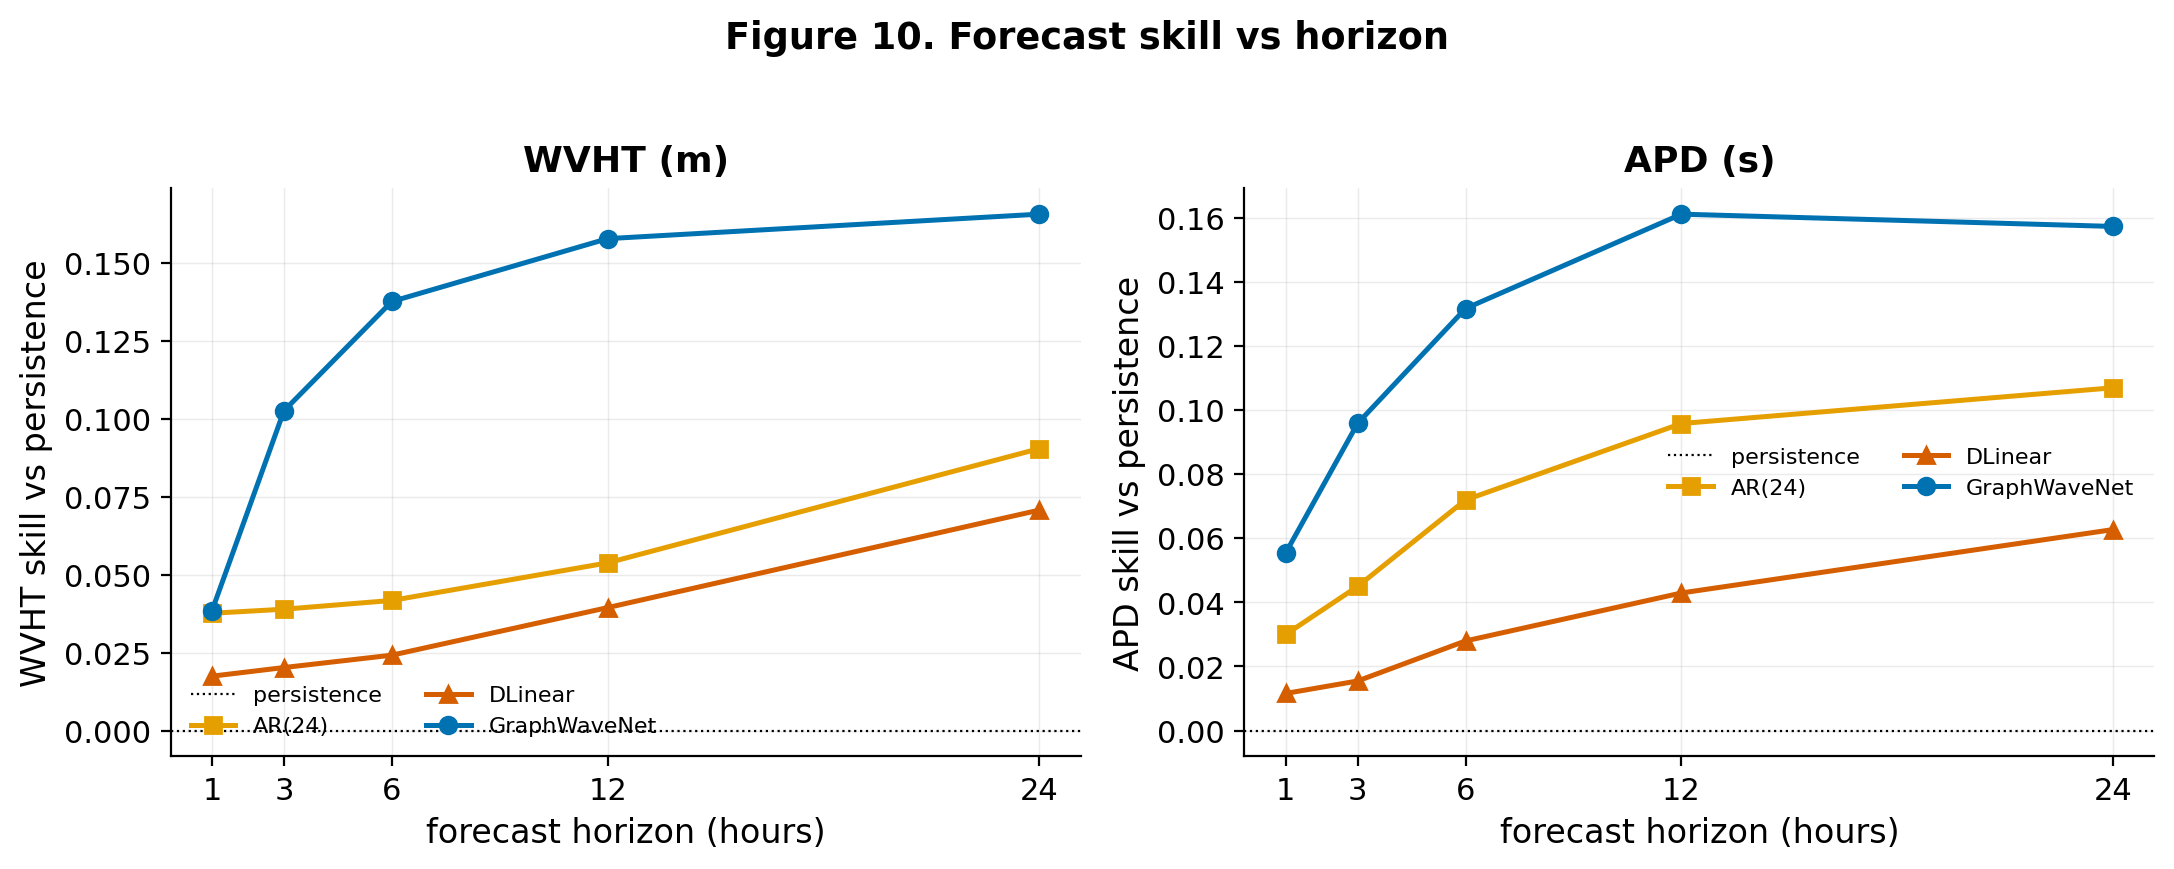
\includegraphics[width=0.86\textwidth]{fig10_horizon_skill.png}
\caption{Forecast skill versus horizon. Persistence saturates at very short
range; the autoregressive model and Graph WaveNet gain skill as the horizon
grows, with the graph model ahead at 12--24~hours.}
\label{fig:horizon}
\end{figure}

\subsection{Wave energy}
Table~\ref{tab:energy} carries the forecasts through Equation~\ref{eq:power} to
wave power, scored on the same leakage-safe origins where both WVHT and APD are
observed. The graph model's advantage not only persists but \emph{grows}. Its
energy-forecast skill is +0.217 at $h{=}12$ and +0.235 at $h{=}24$---
larger than its own height and period skill---while the autoregressive model
reaches +0.111 and +0.164. The reason is the $H^{2}$ nonlinearity in
Equation~\ref{eq:power}: a model that forecasts wave height more accurately earns
a squared benefit in energy, so the graph model's edge on height is magnified in
power. Because $\alpha$ scales all methods equally, these rankings and skills do
not depend on the period-conversion coefficient. Figure~\ref{fig:energy}
summarizes the result.

\begin{table}[t]
\centering
\caption{Wave-energy forecast MAE (kW/m) and persistence-normalized skill (in
parentheses) at 12 and 24 hours, scored where both WVHT and APD are observed.
Rankings and skills are invariant to the period coefficient $\alpha$.}
\label{tab:energy}
\small
\begin{tabular}{l cc}
\toprule
Method & $h{=}12$ & $h{=}24$\\
\midrule
Persistence & 5.468 & 7.691 \\
AR(24) & 4.863 (+0.111) & 6.434 (+0.164) \\
GraphWaveNet & 4.284 (+0.217) & 5.882 (+0.235) \\
\bottomrule
\end{tabular}
\end{table}

\begin{figure}[t]
\centering
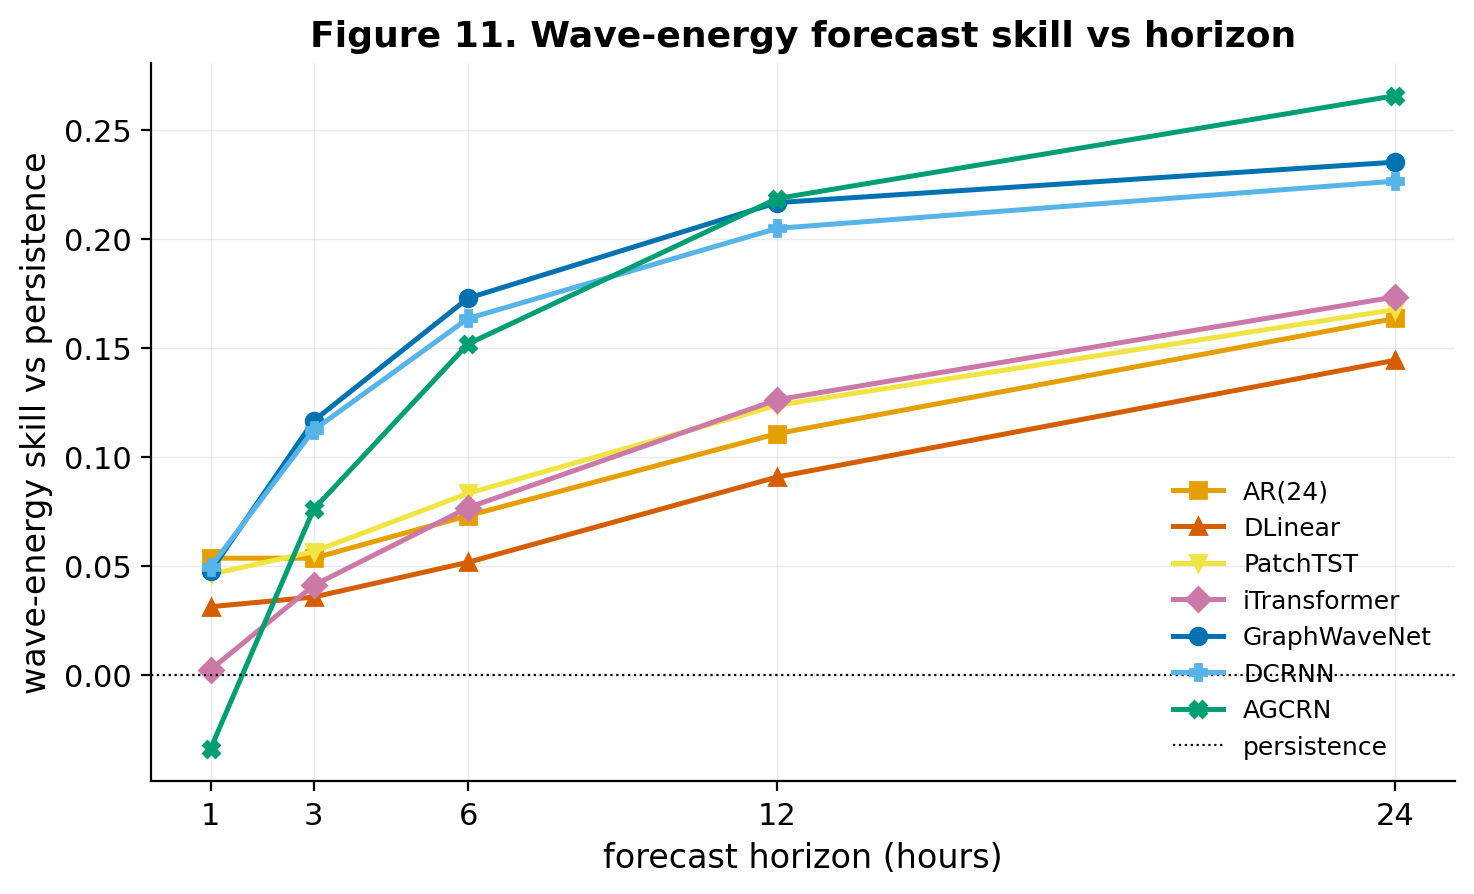
\includegraphics[width=0.78\textwidth]{fig11_energy_forecast.png}
\caption{Wave-energy forecast skill versus persistence. The graph model's
advantage is wider in energy units than in height or period units, because power
scales with the square of wave height.}
\label{fig:energy}
\end{figure}

\section{Discussion}
\label{sec:discussion}
The results tell one coherent story: a spatiotemporal graph helps most where
spatial structure matters most. In imputation this is literal. When a whole
station is missing, its own history is gone and only neighbours can help; the
graph model is the only method that is best here, and the per-station GRIN-minus-
SAITS gap shows the improvement comes specifically from message passing, not from
deep learning in general. When gaps are isolated and random, the advantage
disappears---an isolated missing hour is trivial to interpolate---exactly as one
would expect if the graph's value is the recovery of \emph{structured} loss.

In forecasting the same logic explains both the null and the positive result.
At 1~hour the sea state barely changes, so persistence is near-optimal and there
is little spatial information to add. As the horizon lengthens, swell propagation
between buoys becomes informative, and the graph model converts that propagation
into skill. Carrying forecasts into energy sharpens the picture further: because
power squares wave height, the graph model's height advantage is amplified, and
its energy skill exceeds its height skill. For a practitioner siting a wave-energy
converter, this is the number that matters, and it is where the graph wins by the
widest margin.

We are careful about what we do not show. The basin-aware graph performs within
model-seed noise of the plain graph; rather than bury this, we present it as a
simplification---basin bookkeeping is unnecessary here. The connectivity effect
has the expected sign and some significant coefficients, but with only
$n=38$ victim stations for WVHT (and $n=33$ for APD) it is underpowered, and
we label it suggestive.

\noindent\textbf{Limitations.} Our evaluation is confined to two targets (WVHT
and APD) over one national archive and one multi-year window; other basins,
variables, and periods may behave differently. The energy computation uses a
deep-water approximation and a single period-conversion coefficient; although
rankings are invariant to that coefficient, absolute power magnitudes are not,
and shallow-water sites would need a different flux formula that accounts for
water depth \citep{wang2016}. Deep models were trained under
capped budgets on CPU for reproducibility, not tuned for maximum accuracy, so the
reported skills are conservative. Finally, we benchmark against statistical
baselines, not operational physics-based wave models
\citep{wavewatch3,booij1999};
a hybrid comparison is left to future work.

\section{Conclusion}
\label{sec:conclusion}
We asked whether one modelling idea---a spatiotemporal graph that shares
information between buoys---improves the full applied pipeline for ocean waves.
Across imputation, forecasting, and wave-energy estimation, the answer is yes,
and consistently for the same reason: the graph pays off where spatial structure
is available to exploit. It is the best imputer wherever missingness is
structured---whole-station outages and contiguous blocks---while isolated random
gaps are easy enough that simple interpolation suffices; it adds real 12--24~h
forecast skill over
persistence and autoregression; and it wins by its widest margin on wave power,
where the $H^{2}$ nonlinearity amplifies its superior height forecasts. We also
report where it does not help---a within-noise basin-aware graph and an
underpowered connectivity effect---so that the benchmark is honest about its
limits. Future work should extend the panel, compare against operational wave
models, and add calibrated uncertainty to the forecasts.

\bibliographystyle{plainnat}
\bibliography{main}

\end{document}
